%% Copernicus Publications Manuscript Preparation Template for LaTeX Submissions
%% ---------------------------------
%% This template should be used for copernicus.cls
%% The class file and some style files are bundled in the Copernicus Latex Package, which can be downloaded from the different journal webpages.
%% For further assistance please contact Copernicus Publications at: production@copernicus.org
%% https://publications.copernicus.org/for_authors/manuscript_preparation.html


%% Please use the following documentclass and journal abbreviations for preprints and final revised papers.

%% 2-column papers and preprints
%\documentclass[journal abbreviation, manuscript]{copernicus} % default
\documentclass[gmd, preprint]{copernicus}


%% Journal abbreviations (please use the same for preprints and final revised papers)


% Advances in Geosciences (adgeo)
% Advances in Radio Science (ars)
% Advances in Science and Research (asr)
% Advances in Statistical Climatology, Meteorology and Oceanography (ascmo)
% Annales Geophysicae (angeo)
% Archives Animal Breeding (aab)
% Atmospheric Chemistry and Physics (acp)
% Atmospheric Measurement Techniques (amt)
% Biogeosciences (bg)
% Climate of the Past (cp)
% DEUQUA Special Publications (deuquasp)
% Drinking Water Engineering and Science (dwes)
% Earth Surface Dynamics (esurf)
% Earth System Dynamics (esd)
% Earth System Science Data (essd)
% E&G Quaternary Science Journal (egqsj)
% EGUsphere (egusphere) | This is only for EGUsphere preprints submitted without relation to an EGU journal.
% European Journal of Mineralogy (ejm)
% Fossil Record (fr)
% Geochronology (gchron)
% Geographica Helvetica (gh)
% Geoscience Communication (gc)
% Geoscientific Instrumentation, Methods and Data Systems (gi)
% Geoscientific Model Development (gmd)
% History of Geo- and Space Sciences (hgss)
% Hydrology and Earth System Sciences (hess)
% Journal of Bone and Joint Infection (jbji)
% Journal of Micropalaeontology (jm)
% Journal of Sensors and Sensor Systems (jsss)
% Magnetic Resonance (mr)
% Mechanical Sciences (ms)
% Natural Hazards and Earth System Sciences (nhess)
% Nonlinear Processes in Geophysics (npg)
% Ocean Science (os)
% Polarforschung - Journal of the German Society for Polar Research (polf)
% Primate Biology (pb)
% Proceedings of the International Association of Hydrological Sciences (piahs)
% Safety of Nuclear Waste Disposal (sand)
% Scientific Drilling (sd)
% SOIL (soil)
% Solid Earth (se)
% The Cryosphere (tc)
% Weather and Climate Dynamics (wcd)
% Web Ecology (we)
% Wind Energy Science (wes)


%% \usepackage commands included in the copernicus.cls:
%\usepackage[german, english]{babel}
\usepackage{tabularx}
\usepackage{tablefootnote}
%\usepackage{datetime2}  % \DMTnow
\usepackage[en-GB]{datetime2} % \usepackage[en-GB,en-US]{datetime2}
\DTMlangsetup[en-GB]{ord=raise,abbr,monthyearsep={,\space}}
% https://www.dickimaw-books.com/faq.php?itemlabel=datetime2adjustregional
%\usepackage{hyperref}
%\usepackage{cancel}
%\usepackage{multirow}
%\usepackage{supertabular}
%\usepackage{algorithmic}
%\usepackage{algorithm}
%\usepackage{amsthm}
%\usepackage{float}
%\usepackage{subfig}
%\usepackage{rotating}
%%\usepackage{xparse} %% required for multicite custom function
\usepackage[inkscapelatex=false]{svg} %% use SVG graphics


%% define user commands
\newcommand{\mycomment}[1]{}
% autoref capitalisation
% https://tex.stackexchange.com/questions/34155/autoref-does-not-capitalize-initial-character-in-sentence-when-referencing-labe

% Takes a pair of citations with an optional prefix
% https://tex.stackexchange.com/questions/172699/several-citations-in-the-same-bracket
%\newcommand{\multicite}{ogog}{%
%    \citetext{%
%        \IfValueT{#2}{%
%            \IfValueT{#1}{\citealp[#1;]{#2}}%
%            \IfNoValueT{#1}{\citealp{#2}}%
%        }%
%        \IfValueT{#4}{%
%            ;
%            \IfValueT{#3}{\citealp[#3;]{#4}}%
%            \IfNoValueT{#3}{\citealp{#4}}%
%        }%
%    }
%}

% Define colours to capture author contributions
\def\cred#1{{\color{red}#1}}
\def\cblue#1{{\color{blue}#1}}


\begin{document}

\title{The Coupled Model Intercomparison Project (CMIP): Reviewing project history, evolution, and future}
\mycomment{
was: The Coupled Model Intercomparison Project phase 6 (CMIP6): A review of project evolution and future
Pete G alternate: The Coupled Model Intercomparison Project phase 6 (CMIP6) was made possible by an evolution of project implementation
Jiwoo alternate: The Coupled Model Intercomparison Project (CMIP): a review of project history, evolution and future
}

% \Author[affil]{given_name}{surname} % Author {first initial.}{last}
\Author[1]{Paul J.}{Durack} % ORCID 0000-0003-2835-1438
\Author[1]{Karl E.}{Taylor} % 0000-0002-6491-2135
\Author[1]{Peter J.}{Gleckler} % 0000-0003-2816-6224
\Author[1]{Sasha K.}{Ames} % 0000-0001-9981-2997
\Author[1]{Curt}{Covey} % 0000-0002-0016-7199
\Author[1]{Jiwoo}{Lee} % 0000-0002-0016-7199
\Author[1]{Chris F.}{Mauzey} % 0000-0003-1156-6774
\Author[1]{Jeffrey}{Painter} %?
\Author[2]{Martina}{Stockhause} % 0000-0001-6636-4972
\Author[2]{Michael}{Lautenschlager} %?
\Author[3]{Sandro}{Fiore} % 0000-0002-8430-6087
\Author[3]{Alessandra}{Nuzzo} % 0000-0002-8801-6917
\Author[3]{Fabrizio}{Antonio} % 0000-0002-7693-0111
\Author[3]{Paola}{Nassisi} % 0000-0003-2857-4391
\Author[4]{Matthew}{Mizielinski} % 0000-0002-3457-4702
\Author[5]{Daniel}{Ellis} % 0000-0001-6733-7028
\Author[30,\textdagger]{others please}{add yourselves - will alphabetically reorder once final}

% \affil % Affiliations
\affil[1]{Program for Climate Model Diagnosis and Intercomparison (PCMDI), Lawrence Livermore National Laboratory (LLNL), Livermore, California, USA}
\affil[2]{German Climate Computing Center (DKRZ), Hamburg, Germany}
\affil[3]{Euro-Mediterranean Center on Climate Change (CMCC) Foundation, Lecce, Italy}
\affil[4]{Met Office Hadley Centre (MOHC), Exeter, UK}
\affil[5]{CMIP International Project Office (CMIP-IPO), Oxfordshire, UK}
\affil[30]{Affiliation, location, country}
\affil[\textdagger]{Formerly} %%\textdagger

%% The [] brackets identify the author with the corresponding affiliation. 1, 2, 3, etc. should be inserted.

%% If an author is deceased, please mark the respective author name(s) with a dagger, e.g. "\Author[2,$\dag$]{Anton}{Smith}", and add a further "\affil[$\dag$]{deceased, 1 July 2019}".

%% If authors contributed equally, please mark the respective author names with an asterisk, e.g., "\Author[2,*]{Anton}{Smith}" and "\Author[3,*]{Bradley}{Miller}" and add a further affiliation: "\affil[*]{These authors contributed equally to this work.}".

\correspondence{Paul J. Durack (durack1@llnl.gov)}
\runningtitle{MIP: evolution and future}
\runningauthor{Durack et al.}


\received{}
\pubdiscuss{} %% only important for two-stage journals
\revised{}
\accepted{}
\published{}

%% These dates will be inserted by Copernicus Publications during the typesetting process.

\firstpage{1}
\maketitle


\begin{abstract}
\cred{\textbf{Rewrite once other sections drafted}}

\cred{The CMIP6 project was the most expansive and ambitious Model Intercomparison Project (MIP). Project planning began in 2013, with the first data available in 2018, and new data publication continues today. Over the planning to delivery period, the project grew from 21 to 26 MIPs and from around 190 to 322 experiments defined across them, providing comprehensive coverage of contemporary climate science. Project contributors, primarily modelling groups, also grew considerably in the latest phase, with 45 institutions representing 24 countries providing climate model simulation data to the project. Now that CMIP6 is nearing completion, we review its status, evolution over more than a decade of project planning and delivery, and opportunities and plans for future phases.}

\cred{
\begin{itemize}
  \item Project grew beyond the scope documented in Eyring et al., 2016, which originally defined 190 experiments across 21 MIPs
  \item Phases: planning 2013-2017, operational 2018-present 
  \item Realized potential of distributed Community MIPs
  \item Realization no one modelling system can accurately simulate Earth complexity, with approximations/parameterizations, multi-model approach cross-checks assumptions
  \item "in the end, it is the contributing modelling groups that decide what experiments to prioritize and simulation data to provide for broader community consumption" \citep{stouffer_cmip5_2017}
  \item Built long-standing contributor goodwill and data sharing culture: facilitating groups by providing compute time; tools to aid data creation to meet formats; developing hosting solutions allowing data collation/dissemination; generating projects allowing individual contributions to be uniquely identified, feeding into national and international/IPCC assessments preserving identities to ensure recognition received
  \item "infrastructure delivering the project has become as important as the science that it serves"
  \item Realized the potential of open-access data enabling science discovery and reproducibility
  \item CMIP6Plus and evolution planning underway
  \item Coordinated research led to common language and nomenclature development, enabling an international collaboration targeting the same scientific question with a myriad of modelling approaches following standard experimental and output protocols
  \item History led to community pile-on as MIP standards developed (since AMIP1 facilitated/enabled scientific collaboration)
  \item Economies of scale - set formats/infrastructure once, contribute science multiple times
  \item As MIP momentum has built, the total number of activities and the total number of experiments have grown, reflecting enhanced coordination and community buying into shared and standardized practices
  \item Aspiration to guide infrastructure development through logic that enables more comprehensive model and observational outputs to be uniquely and unambiguously identified, facilitating MIP contributors to generate and downstream data users to access and use these data
  \item VALE Larry Gates
\end{itemize}
} %% end\cred

% Planned submission Wednesday, 27 November 2024.

\cred{
Co-authors to engage
}

\cred{
\begin{itemize}
    \item \textbf{\sout{Jiwoo Lee}, \sout{Curt Covey}, Jeff Painter, Ken Sperber, Ben Santer, Charles Doutriaux, Tom Phillips, PCMDI}: (\autoref{sec:cmip6InContext}: A/CMIP history, \autoref{sec:CMIP6SupportingProjects-CoordEval}: Coordinated evaluation);
    \item \textbf{\underline{Martina Stockhause, DKRZ}} (\autoref{sec:IPCC-DDC}: IPCC DDC; \autoref{sec:DataCitation}: Data citation);
    \item \textbf{\underline{Bryan Lawrence, David Hassell, UReading}}; Eric Guilyardi, IPSL (\autoref{sec:ModelDocumentation}: Model (and data) documentation);
    \item \textbf{\underline{Guillaume Levavasseur, Atef Ben-Nasser, IPSL}} (\autoref{sec:CMIPErrata}: CMIP errata);
    \item \textbf{\underline{Sandro Fiore, CMCC/UTrento}} (\autoref{sec:CMIPDataDownloads}: Data downloads);
    \item \textbf{\underline{Helene Hewitt, John Dunne}, CMIP Panel}: CMIP7 handoff;
    \item \textbf{\underline{Vaishali Naik}}: (\autoref{sec:CMIP6SupportingProjects-input4MIPs} forcing);
    \item \textbf{Sebastien Denvil, Ruth Petrie, CDNOT}: (\autoref{tab:tab1-MIPsThroughTime}/ESGF)
\end{itemize}
}

\cred{
Co-authors/Reviewers to engage: Mon 18 Nov
}

\cred{
\begin{itemize}
    \item \textbf{Jerry Meehl, Ron Stouffer} (CMIP Panel, long-term leadership);
    \item \textbf{\sout{Curt Covey}, Gerry Potter, Dave Bader} (DOE/PCMDI);
    \item \textbf{Dean Williams, Bryan Lawrence, ESGF-XC membership?} (\autoref{sec:CMIPSupportingOrgsAndInfra}: ESGF);
    \item \textbf{Vaishali Naik, Jean-Francois Lamarque, Veronika Eyring}; (\autoref{sec:CMIP6SupportingProjects-input4MIPs}: forcing data CMIP5 through CMIP6);
    \item \textbf{\sout{Curt Covey}, Jerry Meehl, Ron Stouffer, Veronika Eyring, Jean-Francois Lamarque, Cath Senior, Greg Flato, Sandrine Bony}: CMIP Panel
    \item \textbf{Bryan Lawrence, Balaji V., Sebastien Denvil, Luca Cinquini, Mark Elkington, Eric Guilyardi, Michael Lautenschlager, Ruth Petrie, Dean Williams}: WIP Panel
\end{itemize} 
}

{Compiled: \DTMnow}

\end{abstract}

\copyrightstatement{US Department of Energy (DoE) research is considered public domain and can be freely used. When using DoE-supported research, proper attribution to the "US Department of Energy" is requested.} %% This section is optional and can be used for copyright transfers.


\introduction  %% \introduction[modified heading if necessary]
\cred{\textbf{Rewrite once other sections drafted}}

The Model Intercomparison Project (MIP) concept, a well-worn nomenclature in climate science \cred{(Refs)}, has existed for many decades. Among other things, the MIP era has delivered two critical advancements to climate science. The first is that modelling groups contributing to any particular MIP have agreed to make their model output available to be scrutinized by the research community. Before the advent of MIPs, this was generally not the case, as the model analysis was typically performed by individual modelling groups or close collaborators \cred{(Refs)}. The second, contributing to a MIP means agreeing to adhere to a defined experimental design, meaning simulation data could be directly compared.

The acronyms of the Coupled Model Intercomparison Project (CMIP) and Intergovernmental Panel on Climate Change (IPCC) are interchangeably referenced by scientists, stakeholders, and policymakers to refer to the latest climate-model-based science. The MIPs further inspired international effort coordination, leading to considerable science collaboration that has enabled breakthroughs, including the building consensus that human influence is "\textit{unequivocal}" in driving the observed climate changes we are experiencing today \citep[see \autoref{fig:fig6-MIPImpact};][]{eyring_human_2021}. More comprehensive international coordination has marked their development as a way to systematically evaluate observed climate changes, generate plausible future projections driven by varying futures of human development, and assess the fidelity of global climate models (GCMs) and Earth System Models (ESMs) to reproduce past changes and gauge their responses and sensitivities to realistic and idealised climate forcing. The multi-model approach to climate change assessment is now routine, with documented and reproducible experimental protocols and forcing datasets facilitating standardized simulations that can be directly compared across models and with observations to ascertain externally-forced signal from noise and identify robust model responses versus outliers and anomalies that are not representative of our best estimates of the real world.

To provide context for the most recent phase (CMIP6) and the planning of the project’s future, we discuss the efforts dating back to the MIP origins and their contribution to making climate community collaboration what it is today. Small teams or individuals initiated many of the steps taken. While evidence of this history is scattered in literature, we attempt to bring them together to tell a coherent story of how CMIP got to where it is today. Our emphasis details the pragmatics of what it took to progressively scale efforts up, most recently delivering CMIP6, thus this paper describes the evolution of how the MIPs were implemented and the coordinated efforts to establish a minimal infrastructure to make that possible. In \autoref{sec:cmip6InContext}, we discuss MIP phases from 1990 to 2015. In \autoref{sec:cmip6ProjectDesign}, we highlight the CMIP6 experimental design, and in \autoref{sec:CMIPSupportingOrgsAndInfra}, the supporting organizations and infrastructure, \autoref{sec:CMIP6SupportingProjects} describes CMIP6 supporting projects, \autoref{sec:CMIP6Completion} CMIP6 completion and next steps, and conclusions and a look forward to the upcoming CMIP7 phase in \autoref{sec:Conclusions}.

\mycomment{
Mention CMIP6 Community MIPs - mentioned in CMIP5 section.
% Homogenize
Durack+Tayloretal_CMIP6POverview_GMD-CMIP6SpecialIssue
https://docs.google.com/document/d/1Bxu2djLsB0blUUjr4qtwNpZWqMFXkTQRY8kOR_EJvlA/edit?skip_itp2_check=true&pli=1
}


\section{CMIP6 in context with the past}
\label{sec:cmip6InContext}
\cred{\textbf{Attn: Jonathan G., Bryan L; Parallel activities in UK/EU?}}

CMIP6 is the latest in a long history of internationally coordinated climate modelling research projects. The activities grew out of self-organizing communities that built collaborations around science questions and the recognition that systematic multi-model evaluation was needed to build confidence in climate models as effective tools for climate change prediction.

In the United States (US), the scientific motivation for early studies can be linked to coordinated activities organized by the US Department of Energy (DoE), Carbon Dioxide Research Division. In the early 1980s, the DoE CO$_{2}$ Climate Research Plan was established \citep{riches_co2_1983}, which laid out an ambitious proposal to model, detect, and observe CO$_{2}$-induced global and regional climate changes, building on a growing international body of climate science extending back to early seminal works \citep[e.g.,][]{arrhenius_xxxi_1896,chamberlin_attempt_1899,charney_carbon_1979}. The program commissioned a set of six state-of-the-art reports \citep[e.g.,][]{maccracken_projecting_1985} highlighting uncertainties in the current-generation atmospheric general circulation models (GCMs), their simplifications and parameterizations, well ahead of the Intergovernmental Panel on Climate Change (IPCC) program which was endorsed by the World Meteorological Organization (WMO) and United Nations Environment Programme (UNEP) in December 1988. The efforts led to a coordination of international efforts, first establishing the Intercomparison of Radiation Codes used in Climate Models project (ICRCCM) in 1982 \citep{luther_intercomparison_1988,ellingson_intercomparison_1991}, which evolved into a World Climate Research Program (WCRP) and International Radiation Commission joint working group in 1984. The early comparison work highlighted enormous longwave clear sky discrepancies across codes, of order 30-70 W m\textsuperscript{-2}. It led to the recommendation that models needed to be validated against observations to prove their utility, and led to the follow-on Spectral Radiance Experiment \citep[SPECTRE;][]{ellingson_icrccm_1990} co-sponsored by US National Aeronautics and Space Administration \citep[NASA;][]{ellingson_spectral_1996}. Over 22 participants submitted 29 calculation sets to the project, with 7 GCM configurations contributing \citep{ellingson_atmospheric_2016}. The observational design and much of the SPECTRE proposal were subsequently reused to establish the US DoE Atmospheric Radiation Measurement Program \citep[ARM;][]{us_department_of_energy_atmospheric_1990}, initiated in January 1989. Off the back of this early science momentum, in 1984, the DoE initiated the first international GCM intercomparison project to understand the significant differences across CO$_{2}$-forced simulations at the time, the first MIP, FANGIO \citep[see \autoref{sec:amip1And2};][]{ellingson_atmospheric_2016}.

The following sections provide context around the preceding MIPs that led to the latest phase, CMIP6.


\mycomment{
1955-65: Establishment of Atmospheric General Circulation Modelling
http://pne.people.si.umich.edu/sloan/1955_65.html
Establishment of the IPCC UNEP 70th plenary meeting 6 December 1988
https://documents.un.org/doc/resolution/gen/nr0/530/32/img/nr053032.pdf?OpenElement
}

\subsection{Atmospheric Model Intercomparison Project phases (AMIP1/2)}
\label{sec:amip1And2}

Intercomparison of near-term weather, as simulated with different atmospheric models, occurred soon after the first global models were developed in the 1950s \citep[e.g.,][]{gates_ams_1992,edwards_history_2011}. These activities became more coordinated in the early-1970s through the guidance of the Working Group on Numerical Experimentation (WGNE) which was formed in 1967 under the Global Atmospheric Research Program (GARP), a precursor to the World Climate Research Programme (WCRP) \citep{gates_ams_1992}. The first internationally coordinated climate model experimentation occurred in the late 1980s with the scientifically targeted Feedback ANalysis of GCMs and In Observations (FANGIO) project. This project attracted contributions from 19 distinct atmospheric model configurations \citep{cess_methodology_1988, cess_interpretation_1989, cess_intercomparison_1990, cess_first_1991}. The nascent community progress quickly expanded into the first phase of the Atmospheric Model Intercomparison Project \citep[AMIP, hereafter referred to as AMIP1;][]{gates_amip_1992}, which was organized under the purview of the WGNE to help identify systematic errors, narrow the range of model results, and assist in reducing those errors. The acronym AGCM (Atmospheric General Circulation Model) was coined to define model configurations for AMIP, with many of the contributing model configurations also including simplified land-surface representations \citep[e.g.,][]{budyko_heat_1961,manabe_climate_1969,vargas_godoy_global_2021}. AMIP1 provided a community AGCM experimental protocol with time-varying boundary conditions (later referred to as "forcing") of sea surface temperature (SST) and sea-ice for the 1979-1988 period, in addition to the recommended solar constant (1365 W m\textsuperscript{-2}) and carbon dioxide concentration \citep[345 ppm;][]{gates_amip_1991}. It augmented contributing atmospheric model configurations to 27, with 26 community "diagnostic subprojects" established to analyze the simulations \citep{gates_amip_1995}. The project expanded the required model output from simple global and zonal means requested in FANGIO to monthly mean time series (120 covering the 10-year AMIP1 period) in three dimensions. For many participating models, AMIP1 was the first opportunity to run their model longer than one annual cycle, with computer time provided by the Program for Climate Model Diagnosis and Intercomparison (PCMDI; see \autoref{sec:CMIPSupportingOrgsAndInfra}). Early AMIP1 results were assessed in the IPCC First Assessment Report (FAR) \citep{gates_validation_1990}. The successes of AMIP1, including the entrainment of a broader analysis community to assist in model evaluation, motivated the modelling community to revisit the exercise to determine if and how models were improving. To do so, a second phase (AMIP2) was established, including an expanded experimental design with improved boundary conditions \citep{liang_pcmdi_1997, taylor_pcmdi_2000}. The AMIP2 requested Standard Model Output (see \autoref{tab:tab1-MIPsThroughTime} and \autoref{sec:CMIP6DR}) was increased considerably beyond AMIP1, with selected higher frequency data to facilitate process-level analysis. In preparation for AMIP2, an AMIP Panel established by the WGNE reviewed 38 diagnostic subproject proposals \citep{gleckler_amip_2001}, ultimately leading to an interest in comprehensive and systematic model evaluation. As with AMIP1, the AMIP2 community analysis was assessed in the IPCC Second Assessment Report \citep[SAR;][]{gates_climate_1996}, with a focus on assessing mean errors and multi-model consistency across the archive \citep{gates_amip_1995}. The core AGCM experiment pioneered by AMIP1/2 is now a defacto modelling community benchmark experiment that is still frequently used today.


\subsection{Coupled Model Intercomparison Project phases (CMIP1/2/2+)}
\label{sec:cmip1And2And2Plus}

In parallel, work continued at modelling centres to expand model complexity to incorporate a dynamic ocean, amongst other climate system components, which had begun in the late 1960s and early 1970s \citep[e.g.,][]{manabe_climate_1969-1,manabe_global_1975,bryan_global_1975}. The AMIP1/2 experimental protocols, forced with fixed SST and sea-ice, could not simulate future (or past) climate changes. The recognition that climate change can not be fully simulated without properly considering interactions with other major systems, such as the ocean and other missing model components, led to the establishment of the WCRP Steering Group on Global Coupled Models (SGGCM) in November 1990 (\cred{Ref? \href{https://www.wcrp-climate.org/images/AGU2019/presentations/Symposium/11-Meehl_WCRP40.pdf}{Meehl, 2019 AGU WCRP40 presentation} also \href{https://doi.org/10.1093/acrefore/9780190228620.013.933}{Meehl, 2023 OxfordRE}}). Over the following years, the activity entrained oceanographers working in parallel on ocean model development, encapsulated by work hosted by the WCRP CLImate VARiability and Predictability (CLIVAR) project (the CLIVAR Working Group on Ocean Model Development (WGOMD) was subsequently established in 1998). The growing coordination led to the Coupled Model Intercomparison Project (CMIP) acronym being defined and the first phase, CMIP1, designed after a workshop at Scripps Institution of Oceanography in October 1994 \citep{meehl_global_1995}. The acronym AOGCM (Atmosphere-Ocean General Circulation Model) was coined to define model configurations for this project. At the same time, the SGGCM established a small CMIP Panel responsible for planning and providing scientific direction for CMIP, and PCMDI committed to hosting the model output. CMIP1 was focused on collecting data and documenting features of AOGCMs of present-day fixed climate, loosely following the AMIP1 protocol and available forcing data (pdcntrl; see \autoref{tab:tabAppA1-MIPExperiments} for more details). The new community MIP data resource led to considerable community attention and evaluation of the building archive \citep{villwock_6th_2003, lambert_cmip1_2001, raisanen_co2-induced_2001}. In September 1995, the CLIVAR decadal-centennial variations and anthropogenic climate change (DecCen/ACC) Numerical Experimentation Group (NEG-2) was established, which defined an ambitious program of modelling studies, including CMIP \citep{villwock_what_1996, coughlan_report_1996}. The project gathered momentum quickly, with a broad expansion in community-proposed diagnostic subprojects leveraging science insights from the growing archive, and a second phase, CMIP2, was planned and announced in January 1997 \citep{meehl_intercomparison_1997, meehl_coupled_2000}. CMIP2 broadened the science remit, expanding the focus to include a pre-industrial ($\sim$1860) control (picntrl) and climate sensitivity experiments with CO$_{2}$ increasing at 1\% per year \citep[1pctto2x, 1pctto4x;][]{villwock_6th_2003, meehl_cmip_2003}. In parallel to the CMIP growth, there was a recognition that coordinating this activity required a dedicated working group. In April 1997, the WCRP Working Group on Coupled Modelling (WGCM) was created at a CLIVAR Scientific Steering Group (SSG) meeting in Washington DC, reconstituting CLIVAR NEG-2 to meet the growing project needs \citep{detemmerman_clivar_1997} and bringing the project structure and hierarchy inline with what we have in place today. As in AMIP, the CMIP model output received considerable attention with early results included, like AMIP, in the IPCC SAR \citep{gates_climate_1996} and IPCC Third Assessment Report \citep[TAR;][]{mcavaney_model_2001}. With the growing interest in available model data, a recognition was made that the standard output collected to date was only a small subset of model data produced. For the preceding phases, for most variables, time-averaged quantities were collected. In contrast, the time-varying monthly mean information available for a handful of fields (surface temperature, precipitation, and sea level pressure) enabled far broader scientific investigations. Recognizing this opportunity, an augmented phase CMIP2+ was identified and announced in May 2000 \citep{villwock_6th_2003, meehl_cmip_2003, meehl_overview_2005}, with a subset of CMIP1/2 contributing modelling groups augmenting their existing data contributions with considerably more variable and time coverage, including daily data if available \citep{achutarao_pcmdi_2004}.

CMIP2+ enabled research beyond the scope possible with CMIP1 and CMIP2, most notably a comprehensive appraisal of climate models for the US DoE \citep{achutarao_pcmdi_2004}. However, it soon became apparent that contributors and users would greatly benefit from detailed model output specifications--including uniform data formats and standard variable names, units, dimensions, etc. At the same time, the culture of climate-change research had evolved to make open data sharing an expected practice. These two considerations led to the next phase of CMIP, which PCMDI officially agreed to support and host, which was endorsed by the WGCM (representing contributing modelling centres) in October 2003.

\mycomment{
Curt C to provide a sentence or two about the dramatic growth of the registered subprojects that had been the standard engagement way in AMIP1/2, CMIP1/2 and how that
led to the opening up of the CMIP3 archive to open-access FTP, and no registered subprojects? - If I have that right? (already above)

WGOMD establishment after WGCM-2 in Melbourne Oct 1998 - see https://eprints.soton.ac.uk/30149/1/040_wgcm4.pdf#Page=9 /sect3.5 also JSC-21 also see https://www.wcrp-climate.org/modelling-wgcm-publications
CMIP1/2/2+ announcement emails for timing - https://web.archive.org/web/20040827091054/http://www-pcmdi.llnl.gov/cmip/
Also PMIP 1991 - prescribed SSTs AGCMs \citep{braconnot_paleoclimate_2011} \textbf{(Karl to help here)}
Also AMIP2 proceedings, Gleckler et al 2005 - https://pcmdi.llnl.gov/mips/amip/amip2_workshop_proceedings.pdf#page=11 - https://www.osti.gov/biblio/15014509
And Potter 1999 - new strategy beyond AMIP - https://www.osti.gov/biblio/791127
Also Meehl 2019 https://www.wcrp-climate.org/images/AGU2019/presentations/Symposium/11-Meehl_WCRP40.pdf
}


\subsection{Coupled Model Intercomparison Project phase 3 (CMIP3)}
\label{sec:cmip3}

The considerable growth in coordinated MIPs continued throughout the early 2000s and led to the development of what became known as the third phase CMIP3 \citep{meehl_wcrp_2007}. In the early stages, activities that came to define the project were more identified by discrete subprojects, targeting science questions of ocean realism in comparison to observations \citep{orr_ocean_1999, dutay_evaluation_2002, dutay_evaluation_2004} and climate change detection and attribution research targeting the "historical" period \citep{hegerl_20c3m_2003}. Subsequently, many of the initial activities evolved into a more coordinated collection of experiments, which entrained an even greater number of contributing modelling groups. The project saw a step-change across numerous facets, driven by growing and emerging science themes and an increasing appetite by a growing community to access these model data. All contributing models were coupled, simulating the atmosphere, ocean, sea-ice, and, in some cases, the first dynamic land components. By this phase, the flux adjustment, used by many CMIP1/2 contributing models, was largely unnecessary for most contributing AOGCM configurations \citep{durack_ocean_2012}. There was also a dramatic scientific expansion from the fixed pre-industrial control (picntrl) and idealized 1 percent compounding CO$_{2}$ (1pctto2x, 1pctto4x) CMIP1/2 experiments to include for the first time a "Twentieth-century" simulation (20C3M; $\sim$1860-1999), extending from the mid-1800's through until the year 2000, and directly comparable to the growing observational record \citep{meehl_wcrp_2007}. The 20C3M experiment, along with parallel twenty-first century future projection simulations as documented in the Special Report on Emission Scenarios \citep[SRES 2000-2100;][]{nakicenovic_summary_2000} was a step-change for CMIP, for the first time providing model data that could be directly compared to the growing observational datasets, and outlining a project design that would be replicated to great effect in subsequent phases (to become ScenarioMIP in CMIP6). Partial motivation for the 20C3M experiment was to address the growing science around climate change detection and attribution \citep{santer_detection_1996-1, hegerl_20c3m_2003} a research focus that was rapidly expanding since the "..\emph{discernable} human influence on global climate" statement was published in the IPCC SAR \citep{santer_detection_1996}. The explicit recognition that this stage had also identified unforced model internal variability needed to be better understood, and multi-member ensembles (or runs) were encouraged to enable variability quantification \citep{meehl_wcrp_2007}. The project also began incorporating community science, parallel to official CMIP experiments. Notable communities, the nascent Cloud Feedback MIP (CFMIP) established in 2003, which had the single instantaneous CO$_{2}$ doubling (2xco2) and slab ocean (slabcntl) experiments \citep[see also \autoref{tab:tabAppA1-MIPExperiments};][]{mcavaney_cloud_2003, webb_cloud_2017} incorporated as part of the official CMIP3 experiment suite, in addition to Paleoclimate MIP phase 2 (PMIP2) which had been operating in parallel to the A/CMIP phases since 1991 \citep{villwock_6th_2003, braconnot_paleoclimate_2011}. These were just a few of the internationally coordinated activities of the time. At a combined WGCM and International Geosphere-Biosphere Programme (IGBP) Global Analysis Interpretation and Modeling (GAIM) meeting in Canada in 2002, the combined leadership recognized community confusion at the rapid proliferation of MIPs. To better communicate and coordinate activities, a catalogue of MIPs was created on the CLIVAR website, with additions and corrections requested to be sent to the WGCM, GAIM, and CLIVAR Project Office leads, and the last update listing more than 30 unique activities, in addition to AMIP and CMIP \citep{meehl_catalogue_2003}. Like their A/CMIP counterparts, the CMIP3 model output saw even more attention than previous phases. These results, in addition to the body of literature that current and earlier phases of model simulation archives had facilitated, were prominently featured in the IPCC Fourth Assessment Report \citep[AR4;][]{randall_climate_2007}, which itself received the 2007 Nobel Peace Prize \citep{kerr_nobel_2007}.

\mycomment{
CLIVAR MIPs list circa 2005 - lots ~30
http://web.archive.org/web/20050319232556/http://www.clivar.org/science/mips.htm
This omits the CMIP Coordinated Experiment focus which were all announced in 2002 - https://web.archive.org/web/20040827091054/http://www-pcmdi.llnl.gov/cmip/ - subsequently known as CMIP3
Also https://pcmdi.llnl.gov/mips/cmip/ann_20c3m.html
Also PCMDI provided disks to modelling groups who copied data and posted them back - Meehl et al., 2003
Meehl & Hibbard, 2007: A STRATEGY FOR CLIMATE CHANGE STABILIZATION EXPERIMENTS WITH AOGCMs AND ESMs https://www.agci.org/wp-content/uploads/imported-files/2022/07/06S1_WhitePaper.pdf
C4MIP ~2002 https://web.archive.org/web/20040804013119/http://www.c4mip.cnrs-gif.fr/protocol.html
}


\subsection{Coupled Model Intercomparison Project phase 4 (CMIP4)}
\cred{\textbf{Attn: Jerry M., Ron S. representative of reality?}}

While no formal phase was identified CMIP4, some CMIP3 follow-on simulations focused on climate change detection and attribution, specifically single-forcing experiments that held all but one of the 20C3M forcings fixed, were undertaken by several modelling groups. However, these were never formally contributed to a managed multi-model CMIP archive \citep{stouffer_cmip5_2017}. The early effort was a precursor to the CMIP6 Detection and Attribution Model Intercomparison Project \citep[DAMIP;][]{gillett_detection_2016}, building off early work focused on resolving the regional patterns of greenhouse gas and sulphate aerosol forcing \citep{taylor_response_1994, santer_towards_1995, hegerl_optimal_2000, gillett_detecting_2002, hegerl_20c3m_2003}. As planning began for the experiments targeting the next IPCC Fifth Assessment (AR5), aligning the CMIP and the IPCC report phases was an additional motivation to skip the CMIP4 identifier. This additionally also avoided unnecessary confusion with the developing coordinated carbon-cycle modelling activities, with the Coupled Climate-Carbon Cycle Model Intercomparison Project (C4MIP) an active collaborative project of the WGCM and the IGBP that had been running in parallel to the prior CMIP phases \citep{fung_full-form_2000, cox_modelling_2002, friedlingstein_climatecarbon_2006}. C4MIP was one of numerous parallel efforts leveraging science coordination nurtured by the growing MIP community.
\mycomment{
CMIP4 comment - https://www.wcrp-climate.org/images/modelling/WGCM/WGCM17/WGCM17_report.pdf#Page=8
}


\subsection{Coupled Model Intercomparison Project phase 5 (CMIP5)}
\label{sec:cmip5ProjectDesign}

The marked expansion of activities over preceding decades and an ever-expanding data user base led to a considerable project augmentation for its fifth phase (CMIP5). By this stage, many climate research subcommunities had identified MIPs as an effective way to scientifically collaborate, addressing the dual purposes of answering scientific questions through coordinated experimentation and identifying opportunities for model improvement by identifying common errors and biases across the multi-model ensembles. The developing data standards and delivery infrastructure also considerably aided collaboration (see \autoref{sec:CMIPSupportingOrgsAndInfra}), easing access to obtaining and using CMIP output. Planning for the project began in mid-2006 at an Aspen Global Change Institute session which collated representatives across physical climate science, biogeochemistry, impacts and adaptation, and integrated assessment modelling, which laid out needs for near-term and longer-term projection experiments \citep{meehl_introduction_2011}. By CMIP5, the core experiments had been identified, with CMIP core simulations AMIP, piControl, historical (20C3M), 1pctCO2, and an instantaneous CO$_{2}$ quadrupling experiment (abrupt4xCO2) included, targeting model behaviour assessment and climate sensitivity. In addition, the success and attention of the future-focused SRES projections in CMIP3 led to an augmentation of four next-generation Representative Concentration Pathway (RCP) scenarios being defined \citep{moss_next_2010}. The importance of the carbon cycle through land and ocean biogeochemistry had also been recognized, which led to several experiments being included forced with CO$_{2}$ emissions (rather than the imposed atmospheric concentrations of the preceding phases) which depended on Earth System Model (ESM) configurations to contribute \citep{hibbard_strategy_2007,meehl_introduction_2011}.

By 2011, the CMIP5 project design evolution already reflected the more formal MIP structure defined in the following phase (see \autoref{sec:cmip6ProjectDesign}). The CMIP5 "core" experiment set included the diagnostic piControl, AMIP, 20C3M/historical targeting model behaviours, and the 1pctCO2 and abrupt4xCO2 experiments evaluating climate sensitivity, mirroring the CMIP6 "DECK", with the projected future scenarios rcp45 and rcp85 also included \citep{stouffer_cmip5_2011}. The second tier included additional projected future scenarios rcp26 and rcp60 \citep[precursors to CMIP6 ScenarioMIP experiments;][]{hibbard_primer_2011}, CFMIP follow-on experiments including patterned SST experiments sst2030, amip4xCO2, amipFuture, amip4K and along with the aquaplanet experiments aquaControl, aqua4xCO2, and aqua4K \citep{bony_cfmip_2011}, PMIP follow-on paleoclimate experiments included midHolocene, last glacial maximum (lgm) and past1000 \citep{braconnot_paleoclimate_2011}. The project also included experiments targeting short-lived climate forcers sstClimAerosol and sstClimSulfate \citep{boucher_climate_2011}, precursors to CMIP6 AerChemMIP, and the carbon-cycle focused experiments esmrcp85, esmFixClim1, esmFixClim2, esmFdbk1 and esmFdbk2 \citep{friedlingstein_climate-carbon_2011}, precursors to CMIP6's C4MIP. The addition or near-term or initialized prediction experiments was also new to CMIP, with these short-running experiments focused on predicting climate states from the next few years through to a couple of decades \citep{doblas-reyes_cmip5_2011}, identified by the decadalXXXX and noVolcXXXX experiments which in practice worked both in hindcast (back to 1959) and near-term future (to 2015), precursors to the CMIP6 DCPP activity.

\mycomment{
Map CMIP5 experiments to CMIP6 MIPs
https://github.com/PCMDI/CMIP5_CVs/blob/main/src/writeJson.py
https://docs.google.com/document/d/1bUwK6G_fVZO53UjLZbQUOuBP47PsT8lqKKhL1pjRnKg/edit
}


% Migrate figures/data to GitHub repo
% https://www.overleaf.com/learn/latex/Inserting_Images
% https://matplotlib.org/stable/users/explain/figure/backends.html#selecting-a-backend
% https://medium.com/@aaron_imn/a-quick-guide-to-use-scalable-vector-graphics-svg-on-overleaf-ca69448f7177
\begin{figure*}
    \centering
    %\includegraphics[width=1\linewidth]{fileName.png}
    \includesvg[width=1.5\columnwidth]{241118T170837_Fig1.svg}
    \caption{Experiments, models, institutions, and countries contributing to completed Model Intercomparison Project (MIP) phases, from 1989 to today. The project's growth over the most recent phase reflects a growing community appetite for the latest climate data to inform decision-making, a distant evolution from the climate science origin of AMIP1. See \autoref{tab:tabAppA1-MIPExperiments} for an expansion of the experiment lists.}
    \label{fig:fig1-MIPGrowth}
\end{figure*}

%https://tex.stackexchange.com/questions/343028/vertical-centering-of-all-columns-in-tabularx-environment 
\begin{table*}[htp]
\renewcommand{\arraystretch}{1.5}
\scriptsize
\centering
\caption{The Model Intercomparison Projects (MIPs), through time}
\resizebox{\textwidth}{!} {
\begin{tabularx}{0.9\textwidth} {
  | >{\raggedright\arraybackslash}X
  | >{\centering\arraybackslash}X
  | >{\centering\arraybackslash}X
  | >{\centering\arraybackslash}X
  | >{\centering\arraybackslash}X
  | >{\centering\arraybackslash}X
  | >{\centering\arraybackslash}X
  | >{\centering\arraybackslash}X
  | >{\centering\arraybackslash}X
  | >{\centering\arraybackslash}X | }
\hline
\textbf{Planning begins} & \textbf{1989} & \textbf{1993} & \textbf{1995} & \textbf{1997} & \textbf{2003} & \textbf{2008} & \textbf{2013} & \textbf{2022}\\ \hline
\textbf{Project} & AMIP1 & AMIP2 & CMIP1 & CMIP2/2+ & CMIP3 & CMIP5 & CMIP6 & CMIP6+\\ \hline
\textbf{Experiment count} & 1 & 1 & 1 & 2 & 12 & 37 & 322 & $\sim$\\ \hline
\textbf{"historical" period} & 1979-1988 & 1979-2001 & $\sim$ & $\sim$ & $\sim$1860-1999 & 1850-2010 & 1850-2014 & 1850-2022\\ \hline
\textbf{Data volumes} & $\sim$1 GB{}\textsuperscript{\textdagger} & $\sim$500 GB{}\textsuperscript{\textdagger} & $\sim$1 GB{}\textsuperscript{\textdagger} & $\sim$500 GB{}\textsuperscript{\textdagger} & 39 TB & $\sim$2 PB & >27 PB & $\sim$5 PB\\ \hline
\textbf{Standard output variables/ Tables} & 32/4$^{1}$ & 114/8$^{2}$ & 23/5$^{3}$ & 28/5$^{4}$ & 143/6$^{5}$ & 986/18$^{6}$ & 2062/44$^{7}$ & $\sim$\\ \hline
\textbf{Host infrastructure} & PCMDI FTP & PCMDI FTP & PCMDI FTP & PCMDI FTP & PCMDI FTP; ESG-CET & ESGF, \cred{41; Attn: Jeff P., Sebastien D., Ruth P., Sandro F. <2015 records} nodes & ESGF, 30 nodes & ESGF\\ \hline
\textbf{Data formats} & Fortran formatted binary & Fortran formatted binary, GRIB {$\rightarrow$} P-DRS & GRIB {$\rightarrow$} P-DRS & GRIB {$\rightarrow$} P-DRS & CF netCDF-3 & CF netCDF-4 "classic" & CF netCDF-4 & CF netCDF-4\\ \hline
\textbf{Data licenses} & Registered subprojects & Registered subprojects & Registered subprojects & Registered subprojects & Registered subprojects/Open & Open & CC-BY 4.0/CC0 & CC-BY 4.0/CC0\\ \hline
\textbf{Operations begin} & \textbf{1989} & \textbf{1996} & \textbf{1996} & \textbf{1999} & \textbf{2004} & \textbf{2011} & \textbf{2018} & \textbf{2024}\\ \hline
\end{tabularx}
} % /resizebox
\label{tab:tab1-MIPsThroughTime}
\footnotesize{Notes: sources for "Experiment count" are documented in \autoref{sec:secAppA1-MIPExperiments} and \autoref{tab:tabAppA1-MIPExperiments}. {}\textsuperscript{\textdagger}Volume estimates are difficult to quantify, as the provided source and the final archived data differ. GRIB and similar precursor formats were reprocessed to netCDF-3. Sources for "Standard output variables/Tables" noted by superscripts (1-7) are documented in \autoref{sec:secAppB1-MIPStandardOutput} and \autoref{tab:tabAppB1-MIPStandardOutput}. CC = Creative Commons copyright licenses; CC-BY 4.0 = Creative Commons Attribution 4.0 International; CC0 = Creative Commons Public Domain Dedication; for more information, see \url{https://creativecommons.org/share-your-work/cclicenses/}. CF = NetCDF Climate and Forecast Metadata Conventions \citep{eaton_netcdf_2024}. P-DRS = PCMDI Data Retrieval and Storage software library, a precursor to NetCDF. FTP = File Transfer Protocol, a common data transfer protocol. GRIB = General Regularly-distributed Information in Binary format, a precursor to NetCDF, which is still used by the weather community today.}
\end{table*}
% https://www.overleaf.com/learn/latex/Footnotes
%\footnotemark[1]; \footnotetext[1]{AMIP1: Gates, 1991: https://doi.org/10.5281/zenodo.12109765}
\mycomment{
Also WGNE diagnostics, which likely built the original AMIP output list - https://web.archive.org/web/19970825000822/http://www-pcmdi.llnl.gov/amip/output/outlist.html and https://pcmdi.llnl.gov/mips/amip/OUTPUT/WGNEDIAGS/
}

\section{The CMIP6 Project Design}
\label{sec:cmip6ProjectDesign}

When planning for CMIP6 began in 2013, the breadth of science represented and the broad and growing community of contributors and users was recognized. This led to broad community consultation involving the modelling centres whose simulations are the tangible substance of CMIP and the broad and growing communities that rely on CMIP model output for their work \citep{eyring_overview_2016}. The formal development of a core suite of experiments was the result, focused on model evaluation, connecting the activity to the preceding CMIP and AMIP phases. These experiments are referred to as the CMIP6 DECK (Diagnostic, Evaluation, and Characterization of Klima, "klima" being the German word for "climate"). The four primary DECK experiments were named amip, 1pctCO2, abrupt-4xCO2, and the piControl. These, along with a "historical" run and ESM variants of the control and historical experiments (esm-piControl, esm-hist), were typically run by modelling groups during each model development cycle and could not only be used to benchmark model performance but also for comparing different model versions. These were previously considered CMIP5 "core" experiments \citep{stouffer_cmip5_2011}. The interest in special-focus MIPs, now called "Community MIPs", continued, and their number grew to over 20. It was recognized that better coordination was needed to align the growing parallel and sometimes overlapping activities with an awareness of their demands for modelling group resources \citep{eyring_overview_2016}. To address this concern, in planning CMIP6, the CMIP Panel distributed an open call for community MIP proposals in April 2014 to encourage and enhance synergies across activities, reducing duplication and ultimately reducing the burden on contributing modelling groups by standardizing around the common standards and infrastructure that had been developed and delivered in the preceding CMIP5 phase \citep{eyring_overview_2016}. The revised MIP proposals were reviewed in the 2015 Northern Hemisphere summer to prioritize activities that addressed the WCRP Grand Challenges in climate science.

Embodying the federated design, after the \citet{eyring_overview_2016} CMIP6 overview paper was published, MIP growth and additional experiment registrations were received, augmenting the experiment count from 190 to well over 200 experiments \citep{balaji_requirements_2018}. The project growth continued in the following years with two new MIPs, the Climate Dioxide Removal \citep[CDRMIP;][]{keller_carbon_2018} and Polar Amplification \citep[PAMIP;][]{smith_polar_2019} registered in 2018 (see \autoref{tab:tab2-CMIP6MIPs}). During the process of the IPCC AR6 assessment, the development of the COVID pandemic and some additional science questions led to a further augmentation of CMIP6 official experiments, with the Zero Emissions Commitment MIP \citep[ZECMIP;][]{jones_zero_2019} and COVIDMIP \citep{lamboll_modifying_2021} being defined. Their experiments folded into C4MIP and DAMIP, respectively (\autoref{tab:tab2-CMIP6MIPs}). In addition, some sensitivity experiments were also added to the DECK, enabling a single modelling group to contribute simulations comparing the impact of changed climate forcing from CMIP5 to CMIP6 in a single model large ensemble \citep{fyfe_significant_2021}.

At its conclusion, the CMIP6 project included 322 experiments, contributed across 23 MIPs (\autoref{tab:tab2-CMIP6MIPs}). When compared to the prior phases, this order of magnitude growth marked enhanced participation and complexity (\autoref{fig:fig1-MIPGrowth}), capturing an expansion of climate science, and the successful federation of the project structure and management \citep{eyring_overview_2016}.

CMIP6 also embodies changes that occurred as the climate community itself evolved. In early phases, model simulation and analysis were carried out within or in collaboration with a small subset of individual groups. Today, modelling groups develop models and routinely release state-of-the-art model output for public scrutiny, with most of the analysis taking place outside the contributing centres. As such, CMIP planning now involves climate modelling groups, the communities that comprise MIPs and their science foci, and the community of scientists and stakeholders analyzing results. These perspectives are routinely included in ongoing consultation and next-phase planning \citep{stouffer_cmip5_2017}.

While community consultation underpins the CMIP project planning and development to answer pertinent science questions of the day, in the end, it is the contributing modelling groups that decide what experiments to prioritize and simulation data to provide for broader community consumption. Subsequently, the more comprehensive research and stakeholder communities determine what aspects of available model data will be analysed. The CMIP project's central goal is to advance scientific understanding of the Earth system and its responses to ongoing anthropogenic and natural forcing agents. It aims to provide a valuable and tangible resource for national and international climate assessments, including the United Nation's IPCC reports and the Global Stocktake \citep{stouffer_cmip5_2017}.


% https://www.overleaf.com/learn/latex/Tables
% https://www.overleaf.com/learn/latex/Positioning_images_and_tables
% Build history from https://nbviewer.org/github/durack1/MIPPlots/blob/main/CMIPCitationImpact.ipynb

\begin{table*}[htp]
\renewcommand{\arraystretch}{2} % expand table to page size - https://tex.stackexchange.com/questions/8652/what-does-t-and-ht-mean
\scriptsize
\centering
\caption{The CMIP6 Community Model Intercomparison Projects (MIPs), their science focus, and citation}
%\resizebox{\textwidth}{!} {
\begin{tabularx}{1\textwidth} {
  | >{\centering\arraybackslash\hsize=.04\hsize}X 
  | >{\centering\arraybackslash\hsize=.08\hsize}X 
  | >{\centering\arraybackslash\hsize=.33\hsize}X 
  | >{\centering\arraybackslash\hsize=.37\hsize}X 
  | >{\centering\arraybackslash\hsize=.18\hsize}X | }
\hline
\textbf{Count} & \textbf{MIP identity} & \textbf{MIP Description} & \textbf{Science focus} & \textbf{Citation} \\ \hline
1 & AerChemMIP & Aerosol Chemistry & Short-lived climate forcers & \citet{collins_aerchemmip_2017} \\ \hline
2 & C4MIP & Climate-Carbon Cycle & Carbon cycle & \citet{jones_c4mip_2016} \\ \hline
3 & CDRMIP & Carbon Dioxide Removal & Carbon dioxide removal & \citet{keller_carbon_2018} \\ \hline
4 & CFMIP & Cloud Feedback & Cloud feedbacks & \citet{webb_cloud_2017} \\ \hline
5 & CMIP & Diagnostic, Evaluation and Characterisation of Klima (DECK) & Core evaluation, link model evolution across A/CMIP eras & \citet{eyring_overview_2016} \\ \hline
6 & DAMIP & Detection and Attribution & Climate change detection and attribution & \citet{gillett_detection_2016} \\ \hline
7 & DCPP & Decadal Climate Prediction Project & Initialized climate prediction & \citet{boer_decadal_2016} \\ \hline
8 & FAFMIP & Flux-Anomaly Forced & Idealised forced ocean responses & \citet{gregory_flux-anomaly-forced_2016} \\ \hline
9 & GeoMIP & Geoengineering & Geoengineering intervention & \citet{kravitz_geoengineering_2015} \\ \hline
10 & GMMIP & Global Monsoons & Monsoon climatology, variability, prediction and projection & \citet{zhou_gmmip_2016} \\ \hline
11 & HighResMIP & High Resolution & High resolution (<50 km) & \citet{haarsma_high_2016} \\ \hline
12 & ISMIP6 & Ice Sheet & Ice sheet (Greenland \& Antarctica) & \citet{nowicki_ice_2016} \\ \hline
13 & LS3MIP & Land Surface, Snow and Soil moisture & Land-only simulations & \citet{van_den_hurk_ls3mip_2016} \\ \hline
14 & LUMIP & Land Use & Land-use and land-cover change & \citet{lawrence_land_2016} \\ \hline
15 & OMIP & Ocean & Ocean-only simulations (physics) & \citet{griffies_omip_2016} \\ \hline
16 & OMIP & Ocean & Ocean-only simulations (biogeochemistry) & \citet{orr_biogeochemical_2017} \\ \hline
17 & PAMIP & Polar Amplification & SST, sea-ice roles in polar warming & \citet{smith_polar_2019} \\ \hline
18 & PMIP & Paleoclimate & Climate of the deep past & \citet{kageyama_pmip4_2018} \\ \hline
19 & RFMIP & Radiative Forcing & Radiative forcing, transfers and model responses & \citet{pincus_radiative_2016} \\ \hline
20 & ScenarioMIP & Scenarios & Future climate change projections & \citet{oneill_scenario_2016} \\ \hline
21 & VolMIP & Volcanic forcing & Volcanic forcing climate responses & \citet{zanchettin_model_2016} \\ \hline

\multicolumn{5}{l}{\textbf{MIPs (added as an existing MIP subactivity)}} \\ \hline
22 & C4MIP: ZECMIP & Zero Emissions Commitment & CO$_{2}$ emissions and remaining carbon budget & \citet{jones_zero_2019} \\ \hline
23 & DAMIP: COVIDMIP & Modifying emissions to account for COVID-19 & Updated GHG, aerosols, ozone, and optical properties in response to COVID-19 lockdowns & \citet{lamboll_modifying_2021} \\ \hline

\multicolumn{5}{l}{\textbf{Diagnostic MIPs (requesting output from CMIP6 experiments, but having no MIP child experiments)}} \\ \hline
 & WCRP CORDEX & WCRP COordinated Regional Downscaling EXperiment & Regional downscaling related variable request & \cite{gutowski_jr_wcrp_2016} \\ \hline
 & DynVarMIP & Dynamics and Variability & Momentum and energy transport and model bias related variable request & \citet{gerber_dynamics_2016} \\ \hline
 & SIMIP & Sea-Ice MIP & Sea-ice related variable request & \citet{notz_cmip6_2016} \\ \hline
 & VIACSAB & Vulnerability, Impacts, Adaptation and Climate Services Advisory Board & Climate change impacts related variable request & \citet{ruane_vulnerability_2016} \\ \hline
 \textbf{Count} & \textbf{MIP identity} & \textbf{MIP Description} & \textbf{Science focus} & \textbf{Citation} \\ \hline
\end{tabularx}
%} % /resizebox - expands table to larger page format (margin tweaks)
\label{tab:tab2-CMIP6MIPs}
\footnotesize{Notes: MIPs 1 through 21 above are registered in the CMIP6 Controlled Vocabulary (CMIP6\_CVs) GitHub repository, the primary source of CMIP6 registered information. Due to inflexible infrastructure, experiments defined by MIPs 22 and 23 were registered under an existing MIP. \cred{Add number of experiments defined per MIP to meet 322 total?}}
\end{table*}

\section{CMIP supporting organisations and infrastructure}
\label{sec:CMIPSupportingOrgsAndInfra}
\cred{\textbf{Attn: Bryan L. GO-ESSP is mentioned initiated in 2003, I can only find an archived website, and I am not sure how this relates to ESGF. You, Michael, Balaji, Dean, Don etc all listed. Would be useful to get your take - related to this "breakup" that you mentioned}}

The early FANGIO success and the developing appetite to improve climate change understanding led to establishing the Program for Climate Model Diagnosis and Intercomparison (PCMDI) at Lawrence Livermore National Laboratory (LLNL) in 1989. PCMDI was created by the US Department of Energy (DoE) to develop improved methods and tools for the diagnosis, validation, and intercomparison of global climate models. LLNL was selected to host the PCMDI to leverage the co-location of the US DoE Research Scientific Computing Center (NERSC) computing resource (1974-1996) and the pre-existing DoE-supported atmospheric climate modelling efforts that were already underway \citep{potter_celebrating_2011}. The existence of the NERSC high-performance computing infrastructure was one of the significant advantages to the program, enticing 12 international modelling groups to participate in AMIP1 and providing compute cycles to run their codes to develop simulations. These groups ran the ten simulation years (1979-1988), storing their output on the same system \citep{gates_amip_1991, gates_amip_1992}. By 2000, the recognition that the development of supporting infrastructure, data standards, software and hardware that facilitated data delivery to climate scientists, relied upon to serve the growing MIP communities, was now of equal importance to intercomparison, science coordination, and experimental protocols that defined a project with the "I" in the MIP acronym interchangeable across the \textit{intercomparison} and \emph{infrastructure} terms \citep{gleckler_amip_2001}.

Before CMIP5, PCMDI and its collaborators managed all the data distribution responsibilities for AMIP and CMIP. With CMIP5's growth, it became clear that more distributed infrastructure support was needed, and new partnerships were established. To coordinate CMIP technical aspects, in 2014 the WGCM established the WGCM Infrastructure Panel (WIP), which works in parallel and in collaboration with the CMIP Panel to ensure that CMIP data is made widely available. The WIP maintains standards and policies for model data sharing and ensures that the various infrastructure components can be integrated and function smoothly. Its work was critical to the success of CMIP6.

In recent CMIP phases, a number of voluntarily-supported or independently-funded efforts have contributed to various components of CMIP's supporting infrastructure. As described in more detail below, the Climate and Forecast (CF) Metadata Conventions (\autoref{sec:CFConventions}) standardize information used to define and describe all CMIP model output. Controlled Vocabularies (CVs; \autoref{sec:CMIPCVs}) have been established to provide a limited set of terms used to describe and uniquely identify datasets and to aid in searching for data of interest. Additional standardisation is imposed (a process known as "CMORization") by specifying further rules as to data structure and their dimensions, and agreed lists of "standard output" ensure that data reported by different models can be directly intercompared.

Conformance to the standards facilitates management and analysis of the data, which can all be accessed through any of the Earth System Grid Federation (ESGF; \autoref{sec:earthSystemGridFederation}) portals. A subset of the CMIP archive is also replicated by the IPCC Data Distribution Centre (IPCC DDC; \autoref{sec:IPCC-DDC}), which is expected to indefinitely preserve and serve the data. In addition, there have been initiatives to collect and organize model and experiment documentation, to establish a data citation service (issuing DOIs for published datasets), and to make available reports of any errors in existing data. These efforts and services are detailed in the subsections that follow. 

\cred{Is there anything useful in \citet{balaji_requirements_2018}, \citet{petrie_coordinating_2021} \url{http://web.archive.org/web/20180731130715/http://go-essp.gfdl.noaa.gov/}}

\begin{figure*}
    \centering
    \includesvg[width=1.5\columnwidth]{241118T170837_Fig2.svg}
    \caption{Growth of the CMIP6 project over time, with data sizes (PB) identified by colours for each of the CMIP6 Community MIPs (see \autoref{tab:tab2-CMIP6MIPs}) from the initial date of data publication (9th May 2018) through to the latest publication (November 2024). The largest data contributions in CMIP6 are from the CMIP (light blue) and ScenarioMIP (dark grey) activities, comprising 8.4 PB of the >15 PB total. Data growth fluctuated throughout the project's life, with current 2024 publication rates of 2.1 PB/yr (prorated). This compares to previous years: 0.8 in 2023, 3.3 in 2022, 1.8 in 2021, 3.1 in 2020, 3.3 in 2019, and 0.1 PB in 2018.}
    \label{fig:fig2-CMIP6DataGrowth}
\end{figure*}


\subsection{Climate and Forecast (CF) Metadata conventions}
\label{sec:CFConventions}
\cred{\textbf{Attn: Bryan L., David H., Jonathan G. any edits to suggest?}}

By the early 1990s, interest in sharing the output of climate models with researchers outside the originating groups gained momentum. This led to greater attention to clearly defining the model output quantities, ensuring that datasets were self-describing to avoid misinterpretation, standardising their digital formats to ease data transfers and use, and documenting the model configurations that produced the data. In parallel, there were computer science developments focused on generating digital formats that met the needs of growing meteorological data streams, with an aspiration to developing portable and self-describing file formats (where data and metadata that described it were co-contained in files). These developments led to numerous early releases of the network Common Data Format (netCDF) through the late 1980s and early 1990s. In May 1997, netCDF 3.3 was released, which included a new type-safe interface for the C and Fortran languages. In March 2001, netCDF 3.5.0 was released, which integrated a new Fortran90 interface, making this library suitable for integration with climate model libraries primarily written in Fortran \cred{(Refs?)}.
\mycomment{
https://docs.unidata.ucar.edu/nug/2.0-draft/netcdf_history.html
}

In parallel to the netCDF digital format and language interface development, the ability to store rich, self-describing metadata within the file led to considerable work on data conventions. Of climate data relevance, the first was developed by the Cooperative Ocean/Atmosphere Research Data Service (COARDS), a NOAA and US university cooperative aimed at sharing and distributing global atmospheric and oceanographic research datasets. COARDS 1.0 was released in February 1995 and laid out data variable conventions such as assigning spatial dimension/coordinate attributes (height, latitude, longitude) and data variable attributes (long\_name, missing\_value, units), in addition to some required global attributes (e.g., title) providing descriptive context for the data. Much of the COARDS work aided the Ferret visualization and analysis environment development, with Ferret 4.0 released in March 1995 \cred{(Refs?)}. This data standardisation aided the coordination of software efforts, reducing parallel package development into a couple of well-supported packages targeting the evolving COARDS conventions.
\mycomment{
https://ferret.pmel.noaa.gov/Ferret/documentation/coards-netcdf-conventions
https://ferret.pmel.noaa.gov/static/Documentation/Release_Notes/v400.html
Also NCAR CSM - see http://cfconventions.org/conventions.html
}

By 1997, the large and growing MIP archives had accumulated tens of thousands of output files from dozens of model configurations. The diverse and growing international community interested in analyzing and applying results from the models was hampered by the diversity of data formats, structures, and nomenclatures that climate modelling centres had adopted. There would be obvious benefits in standardizing the data. To fill the void, the Gregory, Drach, and Tett \citep[GDT v0;][]{gregory_gdt_1999} standards were first introduced in June 1997. The GDT standard expanded markedly on COARDS, with a prime focus on better enabling GCM output to be self-describing and to conform to standard conventions that made it possible to determine the location of grid cells, the characteristics of the data grid, and interpret time models ("calendar"), climatologies, missing values, and other characteristics essential to avoid misinterpretation. In 1999, the continued development of GDT ceased at v1.4, but the interest it had attracted led to a collaboration of a somewhat larger group of authors who began work developing what became known as the NetCDF Climate and Forecast (CF) Metadata Conventions. Building on and going far beyond COARDS, GDT, and similar efforts, version 1.0 of the CF Conventions was released in October 2003 \citep{eaton_netcdf_2024}.

Subsequently, the CF conventions were adopted by CMIP, starting in phase 3. Since that time, CF gained in popularity across climate sciences and beyond. A formal governance structure was established, and an ever-expanding group of volunteers made contributions extending and correcting flaws in the original conventions (see \url{https://cfconventions.org}). The evolution (while essentially maintaining backward compatibility) has been ongoing through several releases, the latest being version 1.12. The stability of CF, the vibrant community supporting it, and the development of software that can interpret CF data have been foundational to the widespread use of CMIP data. 

\mycomment{
https://www.unidata.ucar.edu/software/netcdf/conventions.html
https://www.unidata.ucar.edu/software/netcdf/coords/proposals.html
COARDS 1995 - https://web.archive.org/web/20100527095818/http://ferret.wrc.noaa.gov/noaa_coop/coop_cdf_profile.html
GDT 1997
https://www.unidata.ucar.edu/mailing_lists/archives/netcdfgroup/1997/msg00080.html
https://www.unidata.ucar.edu/software/netcdf/coords/0054.html 1997
https://web.archive.org/web/20100610102527/http://www-pcmdi.llnl.gov/drach/GDT_convention.html 1999
https://web.archive.org/web/20040604041414/http://www-pcmdi.llnl.gov/drach/netCDF.html
CF 2003 - https://cfconventions.org/Data/cf-conventions/cf-conventions-1.11/cf-conventions.html#_version_1_0_28_october_2003 
}


\subsection{Controlled Vocabularies (CVs)}
\label{sec:CMIPCVs}
\mycomment{\textbf{Attn: IPSL folks; MIP era realm evolution, dovetailing Variable request section}}

As coordinated international climate science activities grew from AMIP1 and 2 through the early CMIP phases, it was recognized that imposing increasingly detailed requirements on the data reported would facilitate its use and increase its value. Early on, it was decided that rather than store multiple variables in a single file, the model output should be organized such that each file contained a single variable. This was done to reduce data download volumes since most analysts of the CMIP data were expected to consider only a small number of variables.

Beginning with CMIP3, each requested variable was assigned a unique name (e.g., “ts” for surface temperature and “pr” for precipitation rate), and all data were written compliant with the CF conventions \citep[e.g.,][]{taylor_pcmdi_2009}. Additionally, the names of the coordinates and their ordering were standardized, and certain CF optional attributes were made mandatory (e.g., "cell\_methods"). Standardisation simplified analysis codes, which could now ingest data produced by multiple models in a common way. In addition, specific metadata were required to be recorded in each file identifying the source of the data (institution, model name, version) and experiment conditions (e.g., experiment name). Thus, the detailed specifications for CMIP3 \citep[see][]{taylor_pcmdi_2005} imposed uniformity on the format and structure of the data and metadata that facilitated its use.

The first collection of controlled vocabularies (CVs) was also introduced in CMIP3 \citep[e.g.,][]{taylor_pcmdi_2005}. In its simplest form, a CV lists the terms used to describe a specific dataset attribute. In CMIP3, there were CVs for variable names (e.g., "tas", "pr", "ua", this subsequently evolved into "standard output" see \autoref{sec:CMIP6DR}), experiments (e.g., "picntrl", "SRESB1", "amip"), institutions and models (e.g., "BCC-CM1", "GFDL-CM2.1", "UKMO-HadGEM1"), and table names (e.g., "O1", "A1", "A2", "A3", see \autoref{tab:tabAppB1-MIPStandardOutput}). The table names identified collections of variables reported at a common "frequency" (1=monthly, 2=daily, 3=3-hourly) and were all associated with either the atmosphere (A) or ocean (O). The CVs were used to construct the directory structure for the data archive, with output from different experiments, models, and variables placed in separate sub-directories. The structure ensured that although the loosely defined template for naming files would not ensure name uniqueness across the entire CMIP3 archive, it would ensure that the names were unique within each lowest-level sub-directory.

The increased uniformity of the CMIP3 data requirements facilitated subsequent research. Still, it burdened modelling groups, who were required to rewrite their data in a new way and a format unfamiliar to some. To assist modelling groups in complying with the model output requirements, the Climate Model Output Rewriter (CMOR1) software \citep{taylor_cmor_2006} along with the CMIP3-CMOR-Tables \citep{doutriaux_cmip3_2005} were developed and made available. In the tables, the 143 requested variables (see \autoref{tab:tab1-MIPsThroughTime}) were grouped so variables likely to be processed under a common procedure appeared together (e.g., ocean and atmosphere variables were found in separate tables). The detailed data specifications and the clearly defined variables were documented in the CMIP3-CMOR-Tables and an "output requirements" document \citep{taylor_pcmdi_2005}. Once the modelling groups prepared their output according to the specifications, it was collected and organized on the PCMDI computing system in an easily searchable directory. The data could be searched and downloaded directly via anonymous ftp or through the ESG web-based data service.

In CMIP5, the trend toward further standardization continued as the project expanded to include additional specialized MIPs, 26 modelling groups, and 37 experiments (\autoref{tab:tab1-MIPsThroughTime}, \autoref{fig:fig1-MIPGrowth}). The original CMOR1 FORTRAN software was revised and recast as C code with FORTRAN and Python interfaces \citep{doutriaux_cmor_2011}. New CMIP5-CMOR-Tables \citep{doutriaux_cmip5_2013} were defined to accommodate the dramatic increase in the variables requested, which now totaled 986 (see \autoref{tab:tab1-MIPsThroughTime}). The data requirements were inherited mainly from CMIP3 but were augmented with additional required attributes, some with values drawn from CVs (e.g., "frequency" and "modelling\_realm").

A major advance in enabling communication among the various components of software infrastructure supporting CMIP5 was the development of a "Data Reference Syntax" (DRS) \citep{taylor_pcmdi_2012}. The DRS relied on several dataset descriptors and associated CVs that uniquely defined each dataset contributing to the CMIP5 archive. The DRS elements were used, for example, in defining the directory structure for the CMIP5 archive and to construct filenames that were guaranteed to be unique across the entire archive. The DRS was also essential for communication and data sharing among the data nodes, which comprised a now federated ESGF data distribution infrastructure \citep{williams_earth_2011}. The DRS dataset descriptors were supplemented with dataset version information assigned during the data preparation and ESGF publication processes, which greatly aided the replication of datasets across the major ESGF federated data nodes.

For CMIP6, the evolution of the data standards, CVs, and supporting infrastructure continued as the project ballooned in size to include 23 specialized MIPs, 49 contributing modelling groups, and 322 experiments (\autoref{tab:tab1-MIPsThroughTime}). Due to the broadening of model diversity and configurations and the concomitant increase in variables of interest, a new approach to defining the data request was tried whereby the needed variables were placed in a database that could be accessed via an API or displayed in different human-readable forms (see \autoref{sec:CMIP6DR}). In total, 2062 variables were requested across all experiments, and these were all transferred into the CMIP6-CMOR-Tables \citep{nadeau_cmip6_2017} and were relied on by a revised CMOR3 \citep{mauzey_cmor_2024} (also see \autoref{tab:tabAppD1-CMIP6PrepTools}).

As new services that enabled formal data citation (see \autoref{sec:DataCitation}) and provided centralized access to extensive model documentation (see \autoref{sec:ModelDocumentation}) began supplementing CMIP's basic service of providing access to CMIP data through ESGF and the IPCC DDC (see \autoref{sec:earthSystemGridFederation} and \autoref{sec:IPCC-DDC}), the CVs became more critical for maintaining consistency across the infrastructure components. The earlier practice of publishing simple human-readable lists of descriptors to identify CMIP datasets had resulted in different parts of the infrastructure replicating this CV information in different specialized formats more suitable for specific purposes. In some cases, the information needed to populate a CV was gathered independently by different components of the infrastructure (e.g., the acronyms used to identify each CMIP experiment), which led to some inconsistency in CV content that hampered transparency and communication across the infrastructure and sometimes confused users of the CMIP data. Consequently, the WIP decided that for CMIP6, a reference repository of CVs would be established, and all infrastructure components would rely on this reference source \citep{durack_cmip6_2024}. The CVs were in JSON files, which humans and machines read easily. Building on the CVs relied on in CMIP5, a few new ones were added. Still, the main advance was providing a definitive source for defining the terms used to uniquely identify CMIP6 datasets and managing them transparently on GitHub.

\mycomment{
old text
As coordinated international climate science activities grew from AMIP1/2 through the early CMIP phases, a parallel growth and refinement of work around the supporting infrastructure and data standards produced relatively stable conventions and common nomenclatures to describe and uniquely identify the various model outputs.

By CMIP3, more than a dozen modelling groups had participated in multiple earlier phases of AMIP and CMIP (\autoref{fig:fig1-MIPGrowth}). The regular contributions of these groups, identified by acronyms naming their institutions and models, identified reasonably consistent file names, which usually included a version number, led naturally to adopting these identifiers to distinguish among the participating models in a way that maintained some continuity across phases. In addition, an abbreviated name was assigned to each of the experiments, now numbering 12 (see \autoref{tab:tab1-MIPsThroughTime}), and the identification of these activities as collections of MIPs (e.g., AMIP, CFMIP, CMIP, PMIP) also allowed experiment acronyms to be created which through NetCDF conventions, allowing for unique identities, filenames, and metadata to be defined. For CMIP3, development of the CMOR1 software \citep{taylor_cmor_2006} along with the CMIP3-CMOR-Tables \citep{doutriaux_cmip3_2005}, organized the 143 variables requested (see \autoref{tab:tab1-MIPsThroughTime}), greatly facilitated the standardization of file metadata that is now common, allowing CMIP3 documentation requirements to be specified \citep{taylor_pcmdi_2005}. For the first time, this enabled modelling groups to describe their data following the guidance and for this data to be organized on the PCMDI computing systems by contributing model, experiment, variable, and CMOR table \citep{doutriaux_cmip3_2005}, which considerably aided the automated replication and organization of the archive.

This process continued in CMIP5, with an increase to 26 modelling groups and an expansion in sub-MIPs leading to 37 experiments making up the phase (\autoref{tab:tab1-MIPsThroughTime}, \autoref{fig:fig1-MIPGrowth}). For CMIP5, the CMOR2 software was developed \citep{doutriaux_cmor_2011} along with the CMIP5-CMOR-Tables \citep{doutriaux_cmip5_2013}, which captured a dramatic increase in the variables requested, now totalling 986 (see \autoref{tab:tab1-MIPsThroughTime}). CMOR2 expanded the standardized metadata that was written to output files, building on the improvements in CMIP3 \citep{taylor_pcmdi_2010}, and in addition imposed standard filenames and directory structures \citep{taylor_pcmdi_2012}, which further aided unique data identities and was necessary to facilitate the growing archives across the now federated ESGF data distribution infrastructure (see \autoref{sec:earthSystemGridFederation}). This phase also incorporated dataset version information, assigned during the data preparation and ESGF publication process, allowing errors to be identified and associated with a data version, greatly aiding more systematic replication and dataset status identity. 

For CMIP6 this evolution continued, with the development of CMOR3 \citep{mauzey_cmor_2024}. The dramatic project expansion with federated sub-MIPs led to a ballooning project, increasing to include 49 contributing modelling groups and 322 experiments (\autoref{tab:tab1-MIPsThroughTime}). Due to the broadening of model diversity and configurations used across this large experimental expansion, a dedicated data request was needed, tying variables requested by MIP/experiment (see \autoref{sec:CMIP6DR}). In total, 2062 variables were requested across all experiments, encoded into the CMIP6-CMOR-Tables \citep{nadeau_cmip6_2017}. Like the phases before it, this led to a further expansion of identifiers and metadata \citep{taylor_pcmdi_2018}, aiding unique data identities and the routine replication of data across the now large international ESGF federation. In addition to CMOR, the community has developed several additional software packages and tools to aid MIP data preparation (see \autoref{tab:tabAppD1-CMIP6PrepTools}).

old notes
For CMIP6, as work on numerous parts of the infrastructure began, their collation of CMIP6 project information occurred independently from one another (ES-Docs, CMIP6 Data Request, and WIP CVs). There was agreement at a WIP meeting in June 2016 (here) that core CMIP6 information needed to be centralized in a single authoritative format for all downstream infrastructure to use, which by that time included the CMIP6 Data Request, ES-Docs, DKRZ Citation Service, ESGF and the modelling-group-serving CMOR and cmip6-cmor-tables. In November 2016, the WIP initiated the first instance of the centralized CVs and developed as the CMIP6_CVs - https://github.com/WCRP-CMIP/CMIP6_CVs. Previous to this, the CMIP6 Data Request (Martin), ES-Docs (Eric Guilyardi and team) and the WIP (Balaji and Karl) had been collating information from the CMIP Panel and MIP Chairs directly. There had been no direct information collation from modelling groups, however, discussions with the CMIP Panel Chair had been ongoing. Once there was a WIP agreement to centralize this information, the activity_id’s, experiment_id’s, institution_id’s and source_id’s were defined (see initial release here), which became the centralized and managed source of information about the CMIP6 project phase, and began the process of harmonizing activity_id/MIP and experiment_id’s across the infrastructure. This also allowed the late registration of new MIPs (CDRMIP and PAMIP in April 2018) and amendments and augmentations to existing MIP experiments, to weed out duplication and more tightly refine the experiment list.

In parallel Martin was working on the CMIP6 Data Request, which began from the information contained in the cmip5-cmor-tables (with familiar table names, e.g., CMIP5_Amon), and built up the CMIP6 variable list which $\sim$doubled over eras (CMIP5 986 to CMIP6 2062). To enable modelling groups to encode their simulation data into the CMIP6 format, CMOR3 was developed with the first 3.0-alpha released on 1 Feb 2016, which required the cmip6-cmor-tables to be defined before this was usable. The cmip6-cmor-tables were first released in June 2017 (here) aligning with version 01.00.11 of the CMIP6 Data Request, with work starting on the CMIP6 Data Request translation in January 2016 (here).
For CMIP6Plus (in preparation for CMIP7) the planning has been to address issues raised with the CMIP6 infrastructure (a high-level overview of the issues are outlined in the CMIP6Plus whitepaper here. Numerous other feedback has been collected over the past years, with some more complete than others, e.g., feedback from CERFACS, CNRM and IPSL here). We have recognized repeating issues over CMIP phases that are far better addressed modularly. After broad consultation, the approach being prototyped through CMIP6Plus_CVs (https://github.com/WCRP-CMIP/CMIP6Plus_CVs) is now in place. The CVs Drop-in, held online on the 8 November 2023 summarised the plans and progress (slides here, other materials here, drop-in report here, recording ?here?). It was an open opportunity for feedback across everyone interested in contributing. Indeed both GitHub repositories are open access, with anyone with a GitHub account able to clone the repo, create issues or submit a pull request with content.
}


\subsection{Variable request and standard output}
\label{sec:CMIP6DR}
\cred{\textbf{Attn: Martin J.}}
\mycomment{Consider realm/frequency evolution across mip eras. RE: realm evolution, started in CMIP3 with tables (A1, O1, etc), built around the history files, from model components - so all ocean history files contained ocean, and sea ice variable, etc - Karl to augment; RE: frequencies, 3D fields, vs 2D fields were separated across tables as these had different temporal requests, to keep request sizes down; \autoref{tab:tab1-MIPsThroughTime} and \autoref{tab:tabAppB1-MIPStandardOutput}

Old: A critical component MIP experimentation is specifying what simulation output to save. It is a trade-off between the efforts required by modelling groups to fulfill a request, available storage, and existing and potential future science needs. Despite advancing technology, saving everything (i.e., all prognostic variables at every timestep) has never been realistic. In AMIP1/2, CMIP1/2/2+/3/5, consideration was made in consultation with MIP chairs and modelling groups about what questions or analyses will be pursued with a given simulation that dictates how much data is saved.

As MIPs emerged, more scientists began analyzing simulations, and it was not always clear a priori what would be studied.
}

For any simulation, models produce fields of climate- and weather-relevant information covering temporal scales from minutes to centuries. Not all information of conceivable interest can be archived due to resource constraints regarding post-processing effort and available storage. Experiment planners must anticipate how essential each model-produced field will be for achieving its objectives and decide whether the fields should be reported at annual, monthly, daily, or sub-daily time-intervals. The challenge is to limit the "standard output" requested from a model experiment to the minimum required and then request, at lower priority, other variables of interest that are not critical to achieving the primary objectives.

In the pre-MIP era (see \autoref{tab:tab1-MIPsThroughTime}), the FANGIO experiments were focused almost entirely on a single objective: to determine whether clouds were responsible for the range of global climate sensitivities found in models. The narrow objective meant that the required output was limited to a few fields and, primarily, to their global means.

When AMIP was proposed, the potential scope of objectives expanded considerably, spanning both time-scales and spatial scales, driven by a growing contributor community. The most popular and readily analysed climate variables were monthly means. Still, even in the early days of AMIP1, scientists were interested in process-level analyses to understand model responses, which required daily or even higher temporal frequency fields.

In AMIP1, storage and resource limitations were a primary concern in defining the "standard output" list. The requested output was agreed upon following extended discussion and negotiation involving the WCRP WGNE, PCMDI, contributing modellers, and other keenly-engaged scientists. Enough temporal mean data was saved to serve the numerous subprojects that were subsequently established to systematically evaluate a diversity of model characteristics \citep{gates_amip_1995}. 

Seeing the interest in AMIP grow, modelling groups realized it would be beneficial to expand the set of model outputs requested to enable a broader range of analyses. Thus, in AMIP2, the standard output more than tripled (from 32 to 114; \autoref{tab:tab1-MIPsThroughTime}) and for the first time included 6-hourly data, which was particularly useful in studying weather phenomena. In addition, the monthly mean covariances needed to evaluate a model's Lorenz energy cycle were reported. These covariances enabled the intended analysis \citep{boer_energy_2008}, but modelling groups felt that given their limited use, the effort required in computing them was unwarranted. Since AMIP2, covariances have not been part of the routine output request and have only been saved for targeted studies.

Compared with AMIP2, CMIP1's standard output list was modest, with just 23 variables requested (\autoref{tab:tab1-MIPsThroughTime}). The sole CMIP1 experiment was a control run focusing on mean climatology, and most variables requested were summer and winter mean fields. There were, however, three multi-year monthly mean surface fields requested: surface air temperature, precipitation, and mean sea level pressure. As in AMIP, the scientists directly involved in organizing CMIP1, primarily the members of the SGGCM/WGCM (see \autoref{sec:cmip1And2And2Plus}) and PCMDI, decided which variables would be archived. Also, as in AMIP, the initial standard output list would inevitably grow over subsequent phases as its scientific impact became apparent.

Although CMIP2 saw only a tiny increase in CMIP's scope, in CMIP3, the number of experiments and the standard output requested increased by more than a factor of five. CMIP3 output was expected to serve an increasingly wide diversity of scientific analyses, and the historical and future scenario experiments would begin serving those studying climate impacts. For such purposes, the variables of most interest to those developing models were augmented with variables characterizing changes near the surface and climate "extreme indices" that might be used to assess impacts. Like the AMIP2 covariance statistics, the requested extreme indices proved challenging to compute and were eliminated from subsequent standard output lists. This set a good precedent for subsequent phases. Still, culling variables from the standard output based on usage statistics should perhaps be pursued more vigorously in future phases even though data popularity is only one of several criteria that must be considered. 

As in earlier phases, the CMIP Panel and PCMDI coordinated the effort to define the CMIP3 output, but input was sought from those with specialized scientific expertise in areas such as clouds (e.g., regarding model variables required for the International Satellite Cloud Climatology Project [ISCCP] simulator needed by those involved in the Cloud Feedbacks Model Intercomparison Project [CFMIP]) or impacts (e.g., regarding extreme indices).

CMIP5 represented a second step change in the size and complexity of the standard output request. The number of experiments tripled to 37, and the number of different variables increased by a factor of 6 to 986 (\autoref{tab:tab1-MIPsThroughTime}). For the first time, CMIP attempted to coordinate the experiments designed by multiple, independently managed MIPs \citep[and all experiments were briefly described by the CMIP5 overview paper,][]{taylor_overview_2012}. As in CMIP3, a common set of standards was imposed on model output. A single comprehensive list of variables was compiled and organized into 6 tables and 13 sub-tables \citep[\autoref{tab:tab1-MIPsThroughTime}, \autoref{tab:tabAppB1-MIPStandardOutput};][]{taylor_pcmdi_2013}. For each MIP experiment defined, whole groups of variables were requested by specifying a subset of the tables; all the variables in a requested table were expected to be reported for specified portions of each simulation (most commonly the entire simulation). Each table contained variables that, with rare exceptions, were all produced by a single model component (e.g., atmosphere, ocean, sea ice, or land) and reported at a single frequency (e.g., 3-hourly, daily, monthly). CFMIP had interest in a number of specialized variables from a small subset of the MIP experiments. Five special tables were defined to meet CFMIP's unique needs (divided into ten sub-tables; \autoref{tab:tabAppB1-MIPStandardOutput}). All CMIP5 tables of variables were accessible as spreadsheets or as machine-readable text files. The mapping of experiments to the tables/variables that were requested could only be done by a person reading the spreadsheet, which poorly served automated data preparation job streams.

For CMIP6, fewer limits were imposed on what experiments and which variables requested would be accommodated. Models were also increasingly becoming more comprehensive, evolving from pure physics to incorporate the atmospheric chemistry and biological components necessary to quantify carbon cycle changes. With more experiments and scientists with varied interests involved and using the downstream data, the requested output became transformed from being defined by a limited but dedicated group of experts guided by the CMIP Panel and PCMDI to one involving more extensive community consultation, including, for example, the many MIP Co-Chairs. The standard output list and the mapping of subsets of the list to particular CMIP6 experiments became known as the "Data Request" \citep{juckes_cmip6_2020}. The exponential growth of MIPs (\autoref{tab:tab2-CMIP6MIPs}) and experiments defined across the phases doubled the total variables requested to 2062 (\autoref{tab:tab1-MIPsThroughTime}). 

The tight timelines imposed on CMIP6 and the complexity of the data request meant that no single individual from a modelling centre (or model component) or those coordinating CMIP infrastructure could provide a careful review of the data request. Consequently, several variables that were difficult to produce or of insufficient interest to warrant being included appeared in the final request. This might partially explain why about 9 percent (i.e., 185) of the CMIP6 variables requested were not subsequently contributed by any of the participating modelling groups. More than a quarter (562 of the 2062 variables) were contributed by two or fewer groups (For comparison, the corresponding numbers in CMIP5 were 40 and 220 under-reported variables of the 986 variables requested). The value of an intercomparison involving results from two or fewer modelling centres is limited, which suggests that when developing future data requests, determining which variables will be reported by modelling groups should receive much more attention. 

\cred{\textbf{Figure capturing requested vs. realized/published data across CMIP3/143 vs ?, CMIP5/978, CMIP6/2062 - can be lifted from the *-cmor-tables/ESGF indexes directly}}

\mycomment{
The CMIP6 "data request" \citep{juckes_cmip6_2020} was the most comprehensively outlined preceded by three decades of evolution in climate model understanding. This history underpinned the development of the standard experimental protocols 
\citet{gates_amip_1991} - AMIP1
\citet{gates_amip_1993} - AMIP History Archive
\citet{gates_amip_1994} - AMIP Ensemble
\citet{gleckler_amip_1996} - AMIP 7 monthly mean and six-hourly output, plus ensembles/AMIP 2
\citet{gleckler_amip_1996-1} - AMIP number 8, STANDARD OUTPUT low and high frequency (6-hr)
https://pcmdi.llnl.gov/mips/amip/OUTPUT/WGNEDIAGS/index.html
\citet{taylor_pcmdi_2009}
\citet{taylor_pcmdi_2013}
\citet{juckes_baseline_2024}

FANGIO not multi-year (perpetual July)/January; AMIP1 success, multi-year SST/sea-ice (Russians and Chinese); AMIP2 next-level output, more high-frequency data, mean products (covariances; u/v-prime overbar - on the fly calculation) monthly mean timeseries (Boer \& Lambert 2008, clim dyn - relationship to Lorenz energy cycle)
CMIP2: https://pcmdi.llnl.gov/mips/cmip2/
CMIP3: https://pcmdi.llnl.gov/mips/cmip3/experiment.html
CMIP5: https://pcmdi.llnl.gov/mips/cmip5/requirements.html
}


\subsection{The Earth System Grid Federation (ESGF)}
\label{sec:earthSystemGridFederation}
\cred{\textbf{Attn: US Dean W., UK/EU Bryan L.; GO-ESSP? Guillaume: Need a paragraph about Synda/and replication in this subsection}}

While addressing current climate science questions through coordinated experimentation is CMIP's core focus, facilitating data access and use by a rapidly expanding international community has become a central project priority. 

For AMIP1/2 and early CMIP phases, the requested standard output was shipped from modelling centres on hard drives or, in some cases, transmitted via FTP to PCMDI. With the goal of facilitating management and analysis, PCMDI developed data formats and software packages for storing and visualizing gridded climate data. Rather than attempt to read data stored in several different native formats and structures, the contributed data was rewritten into the PCMDI "standard" DRS (Data Retrieval and Storage) format, a netCDF file format precursor, and these data were made available to AMIP subproject registrants through a PCMDI file transfer protocol (FTP) server \citep[see \autoref{tab:tab1-MIPsThroughTime};][]{gates_amip_1995}.

By 2000, there was recognition in the US that connecting parallel climate science activities and the associated data archives across institutes could maximize investments across independently funded projects. Besides PCMDI single-site archive of internationally-contributed AMIP and CMIP data, other institutes were beginning to proactively share data.  Activities of this kind were underway at the National Center for Atmospheric Research (NCAR, US) with the Community Climate System Model (CCSM) and the Carbon-Land Model Intercomparison Project (C-LAMP) hosted at Oak Ridge National Laboratory (ORNL, US), and copies of data produced by a number of projects were hosted on the NERSC system at the Lawrence Berkeley National Laboratory (LBNL, US). These groups began ongoing collaborative work developing the federated US infrastructure was prototyped as the "Earth System Grid" \citep[ESG I;][]{bernholdt_earth_2007} supported by DoE, which quickly gathered momentum with additional support from the DoE Scientific Discovery through Advanced Computing (SciDAC) program in 2002 in a second ESG II phase \citep{williams_earth_2009}. By late 2004, ESG II began distributing the CMIP3 data being collated in preparation for the IPCC Fourth Assessment Report (AR4). By the conclusion of CMIP3 in 2009, the 39 terabyte archive of model data had accumulated an order of magnitude more downloads \citep[420 terabytes;][]{ananthakrishnan_building_2007, williams_earth_2009}. Throughout the project lifetime, the hardware hosting the CMIP3 archive had failures, and there was a recognition that the centralized dependence on a single operational system wasn't sustainable long-term, particularly with the parallel growing demand to access and download these data.

By 2006, planning for the IPCC Fifth Assessment Report (AR5) was underway, and with it, CMIP5 (\autoref{sec:cmip5ProjectDesign}). The previous ESG successes led to the development of the next-generation Earth System Grid Center for Enabling Technologies (ESG-CET), which included an expansion of collaborating institutions including Argonne National Laboratory (ANL, US), Los Alamos National Laboratory (LANL, US), National Oceanographic and Atmospheric Administration Pacific Marine Environmental Laboratory (NOAA-PMEL, US) and the University of Southern California Information Sciences Institute (US) \citep{ananthakrishnan_building_2007}, supported by the US DoE Offices of Advanced Scientific Computing Research (ASCR) and Biological and Environmental Research (OBER).

By 2008, infrastructure planning for CMIP5 had commenced, and a recognition was building that connecting international activities to augment the US-centric ESG-CET was needed \citep{williams_global_2016}. An agreement was signed in December 2008 between PCMDI, the British Atmospheric Data Centre (BADC, UK; subsequently Centre for Environmental Data Analysis, CEDA, UK), and the World Data Centre for Climate, German Climate Computing Centre (DKRZ, Germany), identifying the Earth System Grid Federation (ESGF). These two European centres were leads of the IPCC Data Distribution Centre (IPCC DDC), collating and archiving the climate model data used in preparing previous IPCC Assessment Reports. The ESGF goal was to develop a distributed federated architecture that would enable the compute storage resources at each of the centres to facilitate regional modelling groups to publish their CMIP5 model data to one of three nodes and then enable replication of these data across the federation, allowing the users to download or access CMIP5 data from their closest ESGF node \citep{williams_earth_2011}. In addition to the three core centres, additional ESGF nodes were established at the National Computational Infrastructure (NCI, Australia), National Aeronautics and Space Administration Jet Propulsion Laboratory (NASA-JPL, US), NERSC (LBNL, US), ORNL, and NCAR. At the CMIP5 peak, the ESGF had 50 \cred{\textbf{(Clarify numbers of replication/data nodes; Jeff P., Sebastien D.)} active nodes hosting data and software \citep{williams_global_2016}.}
\mycomment{
CMIP6 current nodes - https://aims2.llnl.gov/nodes - 30
Very early CMIP5 http://web.archive.org/web/20111015000202/http://pcmdi3.llnl.gov/esgcet/home.htm 7 nodes ESG-CET + BADC, WDCC, NCI
ESG-CET NCAR, LLNL, ORNL https://extranet.gfdl.noaa.gov/~vb/curator/AR5-20071017/ESG-CET200710.pdf Oct 2007
2013 Aspen workshop - https://www.wcrp-climate.org/images/modelling/WGCM/WGCM17/WGCM17_report.pdf;
Middleton, Foster and Williams et al., 2006: Earth System Grid II final report 2001-2006 SCIDAC https://www.osti.gov/servlets/purl/1113798 https://doi.org/10.2172/1113798
}
\cred{Karl? The ESGF success in delivering CMIP5 led to the CMIP6 planning that began in 2013.. WGCM17}


\subsection{The IPCC Data Distribution Centre (IPCC DDC)}
\label{sec:IPCC-DDC}
\cred{\textbf{Attn: Martina S.;} \citep{stockhause_quality_2012,stockhause_cmip6_2017,stockhause_twenty-five_2022}}

\cred{
Text available \url{https://docs.google.com/document/d/1aQbZj6xQYr-5_Ub9tw9hucm6WzcPIImYMShONPYrpyo/edit}}


\subsection{Model (and data) documentation}
\label{sec:ModelDocumentation}
\cred{\textbf{Attn: Bryan L., David H.}}

\cred{Peter G.: Before model intercomparisons were firmly established community exercises, high-level model documentation was intermittently provided in peer-reviewed publications with more detailed institutional gray literature reports. Early in AMIP, it was recognized that improved documentation could help analysts better interpret their results. A first attempt to coordinate model documentation was made available for the AMIP1 simulations on the PCMDI website \citep{phillips_documentation_1996}}

\cred{David noted WIP telco 241022: CMIP5/Metafor \citep{guilyardi_cmip5_2011} overly constrained [drop down boxes]; CMIP6/ES-Docs \citep{pascoe_documenting_2020} too loosely constrained; CMIP7 EMD this should hopefully hit the sweet spot; Note comprehensive model documentation allows for more quantitative use of data; model genealogy (cf Knutti et al., ${\sim}$2010) can be incorporated into multi-model assessment}


\subsection{Data citation}
\label{sec:DataCitation}
\cred{\textbf{Attn. Martina S.}}

\cred{
With exponential growth in both the climate community using data, and CMIP archive of model output over phases (\autoref{tab:tab1-MIPsThroughTime}), the need to more explicitly assign credit to modelling groups, in addition to uniquely identifying model data used for downstream analyses, tracking errata, and enabling reproducible science, was needed. Before the distributed and federated ESGF development (\autoref{sec:earthSystemGridFederation}), a single location PCMDI hosted the complete AMIP and CMIP archives, but this changed in CMIP5. For this phase, three primary nodes at PCMDI (California, US), The German Climate Computing Centre (DKRZ, Hamburg, Germany), and Centre for Environmental Data Analysis (CEDA, UK), shared the hosting role for the CMIP5 archive - distributed across nodes and not complete at any one centre. Data federation led to a more complex task in keeping track of uniquely identifying datasets. To solve this problem, DKRZ led an effort to both quality control and assign Digital Object Identifiers (DOIs) to CMIP5 datasets \citep{stockhause_quality_2012, stockhause_cmip6_2017}, delivered alongside the long-term archival as part of the DKRZ IPCC Data Distribution Centre \citep[IPCC DDC;][]{stockhause_twenty-five_2022}.}

\cred{
Following CMIP5, for CMIP6, a more ambitious plan was established to meet the needs of IPCC DDC archived data and the evolving data real-time \citep{stockhause_cmip6_2017}. Considering the CMIP project evolution across phases and the federated design that underpinned CMIP6 \citep[see \autoref{sec:cmip6ProjectDesign};][]{eyring_overview_2016}, data citation needed to account for model configurations that were targeted across the 23 MIPs that published data to the project (\autoref{tab:tab2-CMIP6MIPs}). To date, 2,693 CMIP6 DOIs have been generated, with the first issued to the first CMIP6 dataset published in May 2018 (see \autoref{fig:fig2-CMIP6DataGrowth}). CMIP6 DOIs provide two levels of citation support, one targeted at the upper level, a model (source\_id), and another at the lower experiment (experiment\_id) level, allowing a user to more tightly attribute the dataset used.}

\cred{Some information about total citations, persistence, other information, other references?}
\mycomment{
https://www.ipcc-data.org/sim/gcm_monthly/AR5/WG1-Archive.html
https://www.wdc-climate.de/ui/statistics?type=cmip6_doi_registration
https://commons.datacite.org/repositories/8orcv25 - Master overview 6012 citations
https://www.wdc-climate.de/ords/f?p=127:2 - CMIP6 data references
https://www.wdc-climate.de/ui/cmip6?input=CMIP6.ScenarioMIP.NOAA-GFDL.GFDL-CM4.ssp585
https://www.wdc-climate.de/ui/cmip6?input=input4MIPs.CMIP6.CMIP.PCMDI
}


\subsection{CMIP errata}
\label{sec:CMIPErrata}
\cred{\textbf{Attn: Guillaume L., Atef B.-N.}}

\cred{
The growing coherence across successive CMIP archives allowed for more complete data tracking and the development of an errata list documenting user-reported problems. For CMIP3 and CMIP5, user reports via email was captured by PCMDI, and the tabulated information was hosted on an external-facing website and reported to the relevant modelling centre. The slow process yielded a collated error list representing issues across the archive, which led to several data revisions fixing reported issues (see \autoref{tab:tabAppC1-MIPErrata}). For CMIP3, user-reported errors led to the retraction of all simulations from a single modelling centre, as a significant bug was found in the model formulation, rendering its output obsolete.}

\cred{For CMIP6, this process was considerably augmented.}


\subsection{Data downloads}
\label{sec:CMIPDataDownloads}
\cred{Attn: Sandro Fiore}
\cred{
\begin{itemize}
	\item ESG download history and CMIP3 (LLNL/PCMDI; see \autoref{fig:fig5-MIPDownloads})
	\item History of CMCC ESGF involvement
	\item CMIP5 statistics (are CMCC available stats correct back to $\sim$2010?)
	\item CMIP6 statistics
\end{itemize}
}


\section{CMIP6 supporting projects}
\label{sec:CMIP6SupportingProjects}
In addition to the core infrastructure that has delivered past CMIP phases, several uniquely identifiable supporting projects have developed over the past decade. Below is a brief overview of a number of the activities that served CMIP6 or preceding phases.


\subsection{input4MIPs: climate forcing for MIP experiments}
\label{sec:CMIP6SupportingProjects-input4MIPs}
\cred{\textbf{Attn: Vaishali N.}}

As the scientific scope and experiment count broadened through MIP phases (\autoref{fig:fig1-MIPGrowth}, \autoref{tab:tab1-MIPsThroughTime}), the need for climate "forcing" datasets to guide simulation evolution continued to increase. For the initial AMIP1 experiment (1979-1988; AGCM), greenhouse gas concentration and solar irradiance were preset as fixed fields (CO$_{2}$ 345 ppm, and 1365 Wm$^{-2}$ respectively), with time-varying sea surface temperature (SST) and sea ice boundary conditions imposed. As model and experiment complexity increased, more and more complex suites of forcing agents needed to be collated for modelling centre use.

AMIP2 incorporated additional greenhouse gases, ozone, aerosols, and more complex interactive land components \citep[e.g.,][]{gleckler_amip_1996-1,liang_pcmdi_1997}. In CMIP1 and CMIP2/CMIP2+, an interactive ocean and sea-ice removed the need for SST and sea-ice boundary forcing, extending the experiment end date to 2001 (see \autoref{tab:tab1-MIPsThroughTime}).

With the definition of the CMIP3 20C3M/historical experiment \citep[$\sim$1850-2000;][]{meehl_wcrp_2007}, considerable augmentation occurred, with the first historical period datasets hosted by PCMDI alongside existing early AMIP/CMIP data. These data mainly addressed the SRES future scenarios \citep[2001-2100/2200/2300;][]{nakicenovic_summary_2000}, but did include a small number of historical period forcings including those that had already been collated for the AMIP experiment period (1979-2001; \autoref{tab:tab1-MIPsThroughTime}). Additional forcing needs were met independently by each contributing modelling group and model configuration.

For CMIP5, increased model complexity (many models included atmospheric chemistry by this stage) necessitated a far more comprehensive approach to meet the historical experiment forcing needs \citep[1850-2005;][]{taylor_overview_2012}, and to share the workload, considerable coordination across modelling groups occurred. For anthropogenic emissions of short-lived climate forcers (SLCFs 1850-2000; e.g., CH$_{4}$, CO, NOx, etc) dataset creation was led by NCAR, with contributions from a broad community including observationalists and climate modellers \citep{lamarque_historical_2010}. A similar community approach was taken with well-mixed greenhouse gases (WMGHGs; 1765-2300), however, this dataset development was dovetailed with the generation of the RCP future scenario data extending out to 2300 \citep{meinshausen_rcp_2011}. Additional dataset developments contributed to the project fell back to an existing community of researchers who had developed earlier datasets focused on solar variability \citep{frohlich_solar_2004}, volcanic stratospheric aerosol emissions \citep{stenchikov_arctic_2006} and land-use changes \citep{hurtt_underpinnings_2006}. During CMIP5, there was limited standardisation of historical forcing datasets, which differed across modelling groups due to the lack of a centralised and coordinated approach across contributors.

For CMIP6, it was recognised that forcing dataset coordination was needed. The input datasets for model intercomparison projects (input4MIPs) ESGF project was established, and the collation of forcing data required for the CMIP6 DECK experiments commenced. In addition, the collation of additional data supporting 14 other Community MIPs was also published and made available to participating groups \citep{durack_toward_2018}. The input4MIPs project collated next-generation forcing datasets extending from 1850 to 2014 for SLCFs \citep{hoesly_historical_2018,feng_generation_2020}, biomass burning \citep[e.g., fire;][]{van_marle_historic_2017}, land use changes \citep{hurtt_harmonization_2020,chini_land-use_2021}, WMGHGs \citep{meinshausen_historical_2017}, volcanic stratospheric aerosol optical depth \citep[e.g.,][]{aubry_new_2020,aubry_independent_2021,aubry_new_2023}, ozone \citep{checa-garcia_historical_2018}, nitrogen deposition \citep{hegglin_ccmi_2016}, solar irradiance \citep{matthes_solar_2017}, SSTs and sea ice boundary conditions \citep{durack_pcmdi_2018} and anthropogenic aerosol optical properties \citep[e.g.,][]{fiedler_anthropogenic_2019}.

\mycomment{
Over the CMIP phases, ass these forcing datasets became more consistently and routinely produced, some operational weather centres started to pay attention. The European Centre for Medium-Range Weather Forecasts (ECMWF) has used CMIP-era forcing datasets in their ERA5 reanalysis configuration - ERA-Interim, extended to 2019, earlier than CMIP6? - Tim Stockdale/ECWMF); likely similar experience for other agencies JAXA, etc, can this be documented?

CMIP3 NOAA-GFDL experience
\citep{horowitz_global_2003} - MOZART model output - atmos chem/ozone
\citep{olivier_description_1996} - SLCFs/CEDS precursor EDGAR database
\citep{randel_stratospheric_1999} - ozone
\citep{lean_reconstruction_1995,lean_new_2003} - solar
\citep{sato_stratospheric_1993} - volcanic SAOD
\citep{stenchikov_radiative_1998} - volc update
\citep{hansen_efficacy_2005} - climate forcings

CMIP3
https://pcmdi.llnl.gov/mips/cmip/ann_20c3m.html
PCMDI IPCC 4AR simulations and forcing Curt/Karl;
https://web.archive.org/web/20040706074446/http://www-pcmdi.llnl.gov/cmip/
https://web.archive.org/web/20040827091054/http://www-pcmdi.llnl.gov/cmip/
CMIP5
https://pcmdi.llnl.gov/mips/cmip5/forcing.html
NOAA-GFDL history
https://office.wcrp-cmip.org/Products/Files/DocEditor.aspx?fileid=5963 - slide 8 (Vaishali)
Old information CMIP paths
/Users/durack1/sync/Docs/admin/LLNL/12/120607_PaulDurack_PCMDI-CMIP5DataMeeting_LLNL.pdf
/Users/durack1/sync/Docs/admin/LLNL/17/151202_covey1_CMIP1And2/151202_covey1-CMIP1Documentation.pdf
/Users/durack1/sync/Docs/admin/LLNL/17/151202_covey1_CMIP1And2/170530_gleckler1_CMIPPaths.pdf
}


\subsection{obs4MIPs: observations for model evaluation}
\label{sec:CMIP6SupportingProjects-obs4MIPs}

The fundamental role of large-scale, gridded observational products for climate model evaluation was recognized before the advent of organized MIPs. It became a crucial part of the AMIP1 \citep{gates_amip_1992} and AMIP2 \citep{gleckler_amip_1996-1} phases, with a heavy independence on the ECMWF and NCEP/NCAR reanalysis products at that time. Modelling groups and analysts continue collecting observational data for their specific needs, typically ad-hoc, with limited coordination. The obs4MIPs project was established to facilitate model evaluation via the technical alignment of gridded observational products with CMIP standards (see \autoref{sec:CFConventions} and \autoref{sec:CMIPCVs}). It is accomplished by metadata/data integration across projects, facilitating side-by-side data delivery through ESGF (\autoref{sec:earthSystemGridFederation}). The project originated from a PCMDI and NASA collaboration \citep{gleckler_improving_2011} and was later internationalized by the WCRP Data Advisory Council (WDAC; \citep{teixeira_satellite_2014}). An international workshop helped identify critical pathways to improve the effort in preparation for CMIP6 \citep{ferraro_evolving_2015}. Many of these recommendations remain relevant and are being addressed today, for example, with the inclusion of higher frequency, process-relevant gridded data and in-situ station measurements, and a detailed obs4MIPs progress update during CMIP6 was published \citep{waliser_observations_2020}. More recently, obs4MIPs has been revitalized (https://pcmdi.github.io/obs4MIPs) via support of the CMIP IPO, with efforts striving to ensure that obs4MIPs can be a vehicle to accelerate model evaluation, research, and development in future phases of CMIP and related modelling activities. 


\subsection{Coordinated evaluation}
\label{sec:CMIP6SupportingProjects-CoordEval}

AMIP made model output available to analysts with diverse expertise, allowing for more varied and in-depth model evaluation. It established a benchmark against which new and possibly improved models could be evaluated, emphasizing the simulated mean climate and variability assessment on large to global scales. A primary goal was to systematically document errors across a suite of similar models, which had never been done before, and to advance and improve the simulation of physical processes and phenomena \citep{gates_ams_1992}. Recognizing the value of a community-based approach to routine model evaluation, the WGNE created a standard set of mean climate diagnostics (e.g., \url{https://pcmdi.llnl.gov/mips/amip/OUTPUT/WGNEDIAGS/WGNE_Mean_Climate_Diags.pdf}).

By 1994, this philosophy was the explicit science driver behind CMIP1, "intercomparison makes for a better climate model" \citep{meehl_intercomparison_1997}. Since the early days, much progress has been made, with "systematic community evaluation" achieved across every MIP phase since FANGIO. The most prominent examples are the dedicated climate model evaluation chapters that have featured in every IPCC Assessment Report since the FAR in 1990, targeting evaluation of the model generation of the corresponding MIP phase \citep[e.g.,][]{gates_validation_1990,gates_climate_1996,mcavaney_model_2001,randall_climate_2007,flato_evaluation_2013,eyring_human_2021}. As model and evaluation complexity increased, so has the chapter content, expanding from 39 to 130 pages FAR to AR6 \citep{gates_validation_1990,eyring_human_2021}, or including the AR6 model annex \citep{gutierrez_models_2021} and supplementary \citep{eyring_human_2021-1}, 359 pages (noting AR6 Chapter 3 also covered climate change detection and attribution, which in previous reports had a dedicated chapter). The development of internationally coordinated MIP activities naturally nurtured collaborative community evaluation by the active participants, a feature of many activities running parallel to CMIP (e.g., C4MIP, CFMIP, PMIP, etc; C-LAMP: \citeauthor{hoffman_results_2007}, \citeyear{hoffman_results_2007}; Ocean Carbon-Cycle Model Intercomparison Project (OCMIP): \citeauthor{orr_ocean_1999}, \citeyear{orr_ocean_1999}; \citeauthor{dutay_evaluation_2002}, \citeyear{dutay_evaluation_2002}, 
\citeyear{dutay_evaluation_2004}). Outside the IPCC model evaluation chapters, the concept of coordinated evaluation by MIP non-participants was uncommon. With the open access and enhanced standardisation of CMIP3 (see \autoref{sec:CMIPSupportingOrgsAndInfra}), in addition to the availability of model simulations that were directly comparable to the coincident observational record, this led to a more routine and comprehensive evaluation being undertaken. The project advancement nurtured a more diverse and extensive data user group engagement, leading to several seminal contributions that previously would not have been possible \citep{gleckler_performance_2008,eyring_assessment_2006,waugh_quantitative_2008} and which were heavily cited in the subsequent IPCC AR5 model evaluation chapter \citep{flato_evaluation_2013}.

Through CMIP5, this progress continued, with the aspiration of climate model systematic evaluation leading to the development of several dedicated analysis packages targeting the CMIP DECK \citep{eyring_towards_2016}. The ESMValTool \citep[Earth System Model Evaluation Tool;][]{eyring_esmvaltool_2016,righi_earth_2020} is a coordinated European effort that supports the analysis and evaluation of Earth system models by collating a wide array of observational datasets and defining diagnostics that allows for the direct comparison of model simulation output with observations. This effort grew out of the precursor CCMVal-Diags \citep[Chemistry-Climate Model Validation Diagnostic tool;][]{gettelman_community_2012}, which had channelled earlier work \citep{eyring_assessment_2006,waugh_quantitative_2008} into reproducible analysis. The PCMDI Metrics Package (PMP) is another key tool, which built on the pioneering work from CMIP3 \citep{gleckler_performance_2008}, providing a standardized climate model evaluation framework, comparing their outputs with observations curated by the obs4MIPs project across a range of space- and time-scales and variables focused on physical climate mean states and their modes of variability \citep{gleckler_more_2016,lee_systematic_2024}. The ILAMB (International Land Model Benchmarking) package grew out of the earlier C-LAMP activity \citep{hoffman_results_2007} and is focused on assessing the land surface sub-models, offering comprehensive diagnostics and benchmarking to evaluate land-atmosphere interactions \citep{collier_international_2018}. Additional packages that also facilitate and leverage community engagement include the climate process-oriented NOAA Model Diagnostic Task Force \citep[NOAA-MDTF;][]{neelin_process-oriented_2023}, and NCARs Climate Variability Diagnostics Package \citep[CVDP;][]{phillips_evaluating_2014}, amongst numerous others.

These and other community-developed tools (see Hoffman et al., [in prep]) will play increasingly pivotal roles in ensuring climate models are useful tools for climate change prediction and continue to improve through rigorous and systematic community evaluation. It is likely, as the use of CMIP output continues to expand into climate change impacts and adaptation planning, that these tools will be more and more heavily utilized to evaluate simulation data fitness-for-purpose and potentially lead to more advanced methods for model selection and weighting \citep{eyring_taking_2019}.

\mycomment{
Hoffman, F.M., Hassler, B., Beadling, R., Blockley, E., Francis, F., Huang, B., Lee, J., Lembo, V., Lewis, J., Lu, J., Madaus, L., Malinina, E., Medeiros, B., Pokam, W., Scoccimarro, E., Swaminathan, R., and Marquez, A.L., 2024. Systematic Benchmarking of Climate Models: Methodologies, Applications, and New Directions [to be submitted soon]

The history continues back into the early 1990s, e.g., PILPS (The project for Intercomparison of land surface parameterisaton schemes PILPS) Henderson-Sellers et al., 1995, see 
https://www.wcrp-climate.org/modelling-wgcm-mip-catalogue/modelling-wgcm-mips-2/268-modelling-wgcm-catalogue-pilps

Also https://www.wcrp-climate.org/modelling-wgcm-mip-catalogue/modelling-wgcm-mips (18), and https://www.wcrp-climate.org/modelling-wgcm-mip-catalogue/modelling-wgcm-mips-2 (1:10, 2:10, 3:10, 4:7)

Jiwoo's original text - CMIP7 future focus, migrate to Dunne et al?

Model evaluation and benchmarking are crucial in assessing climate models, helping to quantify their performance and identify areas for improvement. Over the years, several tools have been developed to streamline this process, particularly in the context of the CMIP (Hoffman et al., 2024 [in prep]). The PCMDI Metrics Package (PMP) is one of the key tools, providing a standardized framework for evaluating climate models by comparing their outputs with observations from obs4MIPs across a range of variables focusing on physical climate and their variabilities \citep{gleckler_more_2016,lee_systematic_2024}. ILAMB (International Land Model Benchmarking) focuses on assessing land surface models, offering comprehensive diagnostics and benchmarking to evaluate their representation of land-atmosphere interactions \citep{collier_international_2018}. Similarly, the ESMValTool (Earth System Model Evaluation Tool) supports the analysis and evaluation of Earth system models by incorporating a wide array of observational datasets and diagnostics, enabling multi-model comparisons \citep{eyring_overview_2016}. These and other tools available in the community as reviewed by Hoffman et al. (2024) play pivotal roles in ensuring that models participating in CMIP meet rigorous scientific standards, facilitating ongoing model improvement and fostering transparency in model evaluation. Together, they have significantly advanced the field of climate model assessment, contributing to the evolution of CMIP phases by providing quasi-operational evaluation capabilities, for example, as demonstrated in the past IPCC AR reports \citep{mcavaney_model_2001,flato_evaluation_2013,eyring_human_2021}.

To leverage these tools more efficiently and immediately, the WCRP established the Climate Model Benchmarking Task Team to provide a systematic and rapid performance assessment of CMIP models, particularly for the expected CMIP7 participating models. The Task Team proposed the concept for a new Rapid Evaluation Framework (Hoffman et al. 2024 [in prep]), whose development is initiated and in progress for CMIP AR7 Fast Track simulations to support the next IPCC Assessment Report 7 (AR7) cycle.
}


% Migrate figures/data to GitHub repo
\begin{figure*}
    \centering
    \includesvg[width=1.5\columnwidth]{241118T170837_Fig3.svg}
    \caption{Web of Science citations for key overview papers of all MIP phases, from FANGIO \citep{cess_intercomparison_1990} through CMIP6, both the project overview paper \citep{eyring_overview_2016}, each of the community MIPs that comprise the phase (see \autoref{tab:tab2-CMIP6MIPs}) and a composite of these two sources from their publication to today. Citation counts are an imperfect way to capture MIP impact but reflect a large and strongly growing user community using MIP data across numerous phases.}
    \label{fig:fig3-MIPPhaseCitations}
\end{figure*}

% Migrate figures/data to GitHub repo
\begin{figure*}
    \centering
    \includesvg[width=1\textwidth]{241118T170837_Fig4.svg}
    \caption{Web of Science citations for the 23 MIPs contributing to CMIP6 (see \autoref{tab:tab2-CMIP6MIPs}) from their publication to today. Black text numbers on each coloured bar denote citation counts. Citation counts are an imperfect way to capture MIP impact. Still, they are reflective of the large interest in the future climate change projections captured by ScenarioMIP \citep{oneill_scenario_2016} and the high-resolution simulations captured in HighResMIP \citep{haarsma_high_2016}.}
    \label{fig:fig4-MIPCitations}
\end{figure*}

% Migrate figures/data to GitHub repo
\begin{figure*}
    \centering
    \includesvg[width=\textwidth]{241118T170837_Fig5.svg}
    \caption{Downloads across the three phases of CMIP, for which records are available. Each horizontal stacked plot represents total download counts as percentages from 2018-November 2024 for CMIP5 and CMIP6, and 2004-2008 for CMIP3. For display, all ScenarioMIP experiments (CMIP3: SRES; CMIP5: RCP; CMIP6: SSP) are presented as cumulative totals across all contributing experiments, with other results displaying single experiment downloads. Top, the CMIP3 \citep{meehl_wcrp_2007} downloads across the top 6 experiments (3x ScenarioMIP) of 12 experiments total (see \autoref{tab:tabAppA1-MIPExperiments}), representing 94.3\%. Middle, the CMIP5 downloads across 9 experiments (4x ScenarioMIP), representing 88.7\%, of 37 experiments that defined the phase \citep[representing 8 MIPs identified in \autoref{tab:tabAppA1-MIPExperiments};][]{taylor_overview_2012} (\cred{Sandro F., can these numbers, obtained Nov 2024 be relied upon to represent the full 2010-2018 CMIP5 project downloads?}). Bottom, the CMIP6 downloads across 12 experiments (8x ScenarioMIP), representing 86.6\% representing 20 MIPs that published data to ESGF (see \autoref{tab:tab2-CMIP6MIPs}). For CMIP6, almost 50\% of downloads were accounted for by the 7 core CMIP/DECK simulations \citep{eyring_overview_2016}, with 34\% accounted for in the 8 ScenarioMIP future projection experiments \citep{oneill_scenario_2016}. This pattern of data download priority is mirrored across the prior phases, with an inversion in CMIP5 (ScenarioMIP 44\%, CMIP 41\%) and a more dominant 20C3M/picntrl demand in CMIP3 (CMIP 64\%, 35\% ScenarioMIP). \cred{Appetite to tabulate results?}}.
    \label{fig:fig5-MIPDownloads}
\end{figure*}

% Migrate figures/data to GitHub repo
% https://superuser.com/questions/415707/export-excel-graphs-as-vector-graphics-files-e-g-svgs
\begin{figure*}
    \centering
    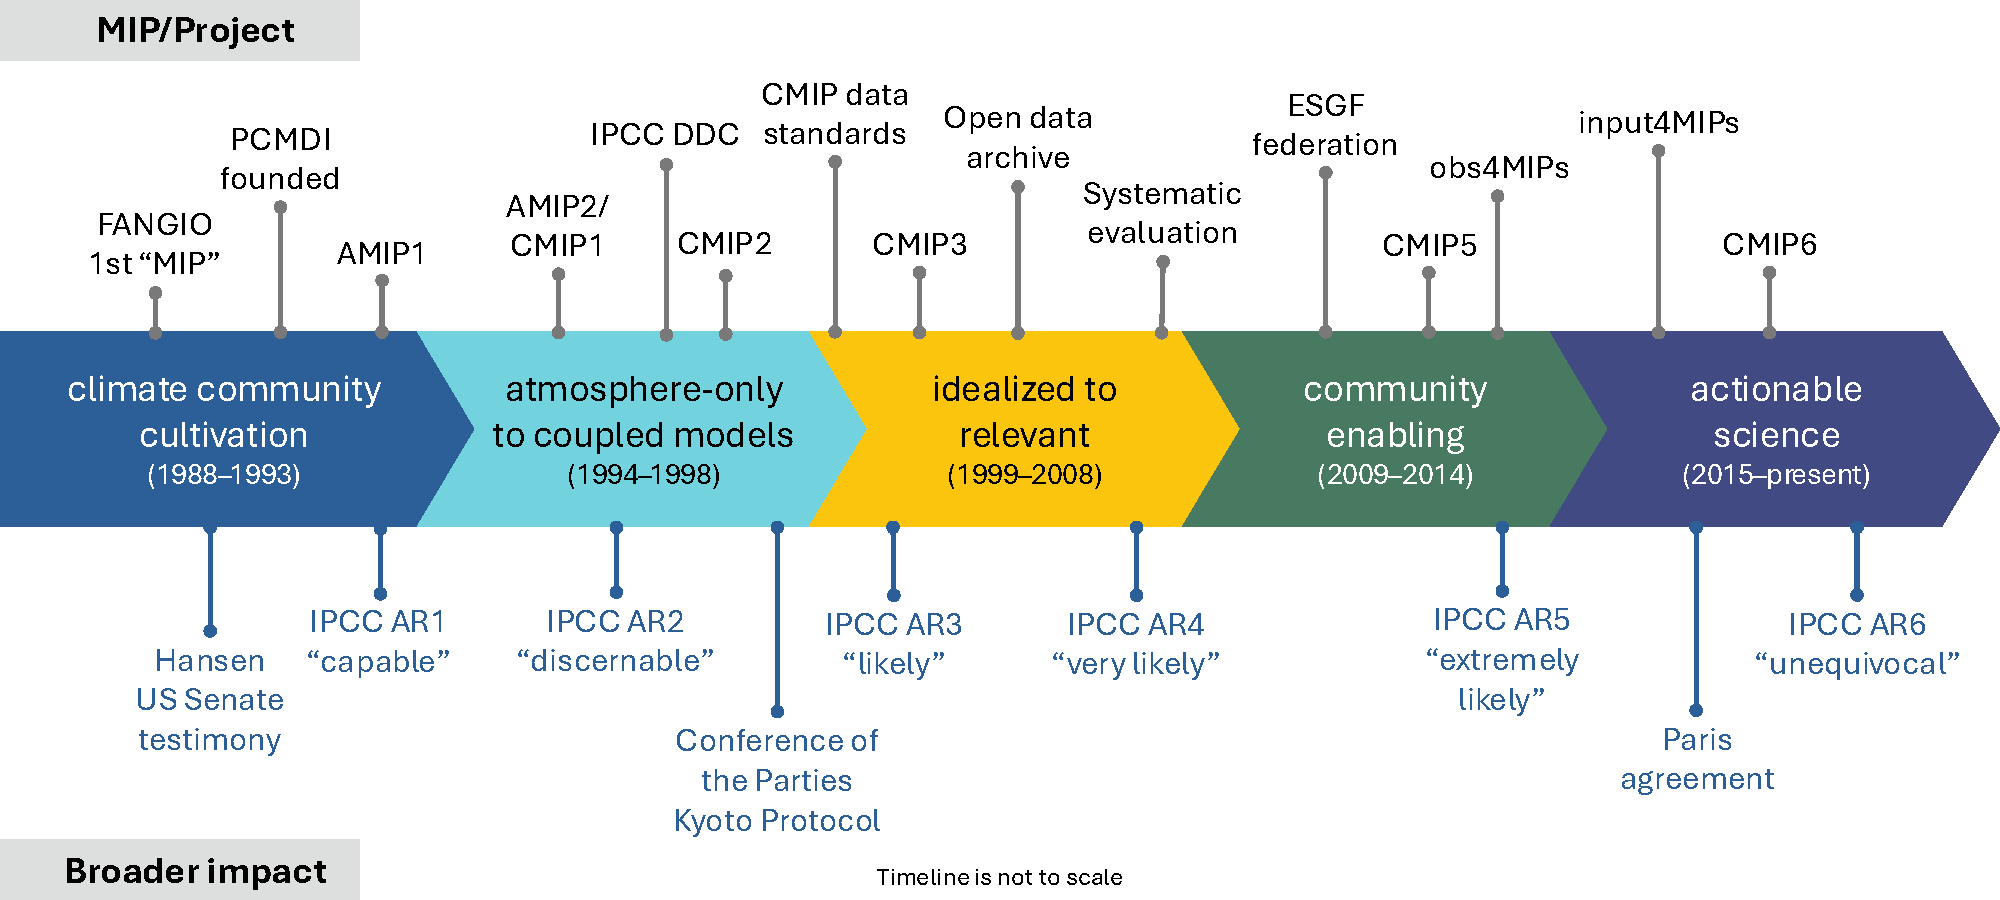
\includegraphics[width=\textwidth]{241119T110937_Fig6.pdf}
    \caption{A time history of MIPs and their broader impact, with particular relevance to the IPCC Assessment Report phases and statements of human influence on the climate (in parentheses, FAR through AR6; see \autoref{sec:amip1And2} through \autoref{sec:cmip6ProjectDesign}). \cred{ESG I, II, missing, what else?}}
    \label{fig:fig6-MIPImpact}
\end{figure*}


\section{CMIP impact and CMIP6 completion}
\label{sec:CMIP6Completion}
\cblue{\textbf{COMPLETE OUTLINE - Tue 19 Nov}}

For a project like CMIP, which has evolved markedly over its four decades of operation, it is challenging to accurately quantify its impact, apportion recognition to its contributors and participants, and identify the breadth and diversity of users of generated data downstream. Moving to an open data paradigm (and equivalent open data licenses, \autoref{tab:tab1-MIPsThroughTime}) with CMIP3, further complicated project attribution, leading to mirror sites creating secondary data repositories outside the ESGF licensing and access control \citep[e.g.,][]{balaji_requirements_2018}. In addition, compute services co-located with the primary ESGF replication nodes (e.g., PCMDI, DKRZ, and CEDA), other regional nodes (e.g., NCAR, NCI) and the replication of datasets into the commercial cloud \citep[e.g., PANGEO;][]{abernathey_cmip6_2020} began to serve larger and more diverse online communities, further complicating the assessment of data access and use.

CMIP data is now routinely used outside the physical climate science community and, more broadly, outside the academic community. This is a dramatic shift from the FANGIO/AMIP early days, which began the climate model intercomparison activities that involved the modelling group participants alone. Consequently, academic literature citations are an imperfect metric for quantifying impact. Regardless, as a representative "overview" paper exists for each phase, it is useful to evaluate MIP phase impact per citation dating back to the earliest publication \citep[FANGIO;][]{cess_intercomparison_1990}. To place citations in context, the seminal work of the \citep{charney_carbon_1979} report has also been included, which was one of the first reports that included idealised climate change predictions from climate models (two US, NOAA-GFDL and NASA-GISS, and one from the UK MetOffice). The \citet{charney_carbon_1979} report was published by the US National Academy of Sciences, and consequently time-evolving Web of Science citation counts are not available, and rather just a single cumulative citation count from Google Scholar (see \autoref{fig:fig3-MIPPhaseCitations}).

\cred{
\autoref{fig:fig3-MIPPhaseCitations} citations per MIP phase, \autoref{fig:fig4-MIPCitations} citations per CMIP6 Community MIP, \autoref{fig:fig5-MIPDownloads} CMIP data downloads per experiment across the CMIP3, CMIP5 and CMIP6 phases, and \autoref{fig:fig6-MIPImpact} an attempt at documenting the broader impact of climate science chronologically aligned with the MIP phases that anchored the science on which these IPCC assessments, and community agreements were made.
}
\cred{
Downloads, citations.. imperfect measures of impact, but relevant measures of community interest in Community MIPs and their experiments.

CMIP6 30 data nodes publishing data, 9 reporting download statistics
CMIP5 $\sim$35 data nodes publishing, 7 reporting download statistics (all CMIP6 data nodes)
}
\cred{
In the end, it is the contributing modelling groups that decide what experiments to prioritize and simulation data to provide for broader community consumption
}
\cred{
CMIP6 closure, CMIP6Plus continuation as interim phase, allowing MIPs to continue to leverage infrastructure while preparation for CMIP7 occurs (with infrastructure overhaul)
}

\cred{Pull/harmonize items from abstract section; Coordinated activities, ESMO benefits from model side well organized, no organize obs. Obs community have model targets to aspire to aid, higher resolution observations - target observations for model evaluation?}


\cred{
\begin{itemize}
	\item Broad community consultation
	\item Larger, more coordinated activities
	\item Still dependent on infrastructure providers (engaged since CMIP3) to deliver the project
\end{itemize}
}


\section{Conclusions and next steps} %% \conclusions[modified heading if necessary]
\label{sec:Conclusions}
\cred{\textbf{awaiting sections to be written above}}

\cred{\textbf{John D., Helene H. handoff}}

\cred{Call out \citet{shukla_strategies_2009,shukla_toward_2010}, \citep{jakob_need_2023}, \citep{stevens_perspective_2024} commentary papers highlighting "operational" vs "science innovation" pressures have been growing across phases}

Planning is underway for a future CMIP7 phase, with the expectation that project data will become available in 2025. Following the CMIP6 broad expansion, CMIP7 will likely further federate discrete activities and encompass climate model simulations from an even broader contributor pool. Infrastructure providers are undertaking considerable updates to modernize the supporting hardware and software for project delivery to facilitate the transition. In preparation for the transition, continued publications to the CMIP6 archive will cease in early 2025, with the project sunsetting soon after that. CMIP6 data will continue to be made available through the federated ESGF network, however, the priority for data curation and maintenance will shift in favour of CMIP7 soon after the first datasets become available.

\cred{John D.: As planning continues for the 7th phase of CMIP \citep{dunne_climate_2024}, it draws from a rich legacy of international cooperation and increasing community engagement with lessons learned from decades of dedicated efforts to optimize the value and utility of model data for climate model systematic evaluation and diverse applications.}

\cred{GMD CMIP7 Special Issue; GMD CMIP7 Forcings Special Issue; Infrastructure concepts of multiverse/CMIP, planet/project and continent/user}

\cred{
\begin{itemize}
	\item Need for CMIP IPO identified in 2019 and open call for tenders
	\item CMIP IPO awarded 2021
	\item Aiding broad community engagement and formalization of governance, allowing the development of Task Teams to meet CMIP7 planning needs
	\item $\sim$35 MIPs self-identified - see MIP rego page \citep[LESFMIP;][]{smith_attribution_2022}, \citep[RAMIP;][]{wilcox_regional_2023}, \citep[CERESMIP;][]{schmidt_ceresmip_2023}, TIPMIP \citep[][]{winkelmann_tipping_2023}, TBIMIP \citep[][]{richter_tropical_2024}, ...
    \item Fresh eyes, early career engagement
\end{itemize}
}


%% Following commands are statements for data sets and/or software code availability corresponding to the manuscript.
%% Use these sections if data sets and/or software code are part of what your research article is based on.

%\codeavailability{TEXT} %% use this section when having only software code available

%\dataavailability{TEXT} %% use this section when having only data sets available

\codedataavailability{Data underpinning figures in the paper, in addition to tabulated additional information can be viewed in a paper-dedicated GitHub repository at \url{https://github.com/durack1/CMIPSummary}, or online using NBViewer at \url{https://nbviewer.org/github/durack1/CMIPSummary/blob/main/figuresAndTables.ipynb}.} %% use this section when having data sets and software code available

%\sampleavailability{TEXT} %% use this section when having geoscientific samples available

%\videosupplement{TEXT} %% use this section when having video supplements available

\appendix
\section{Defined experiments across MIP phases}  %% Appendix A
%\subsection{}     %% Appendix A1, A2, etc.
\label{sec:secAppA1-MIPExperiments}
There is considerable continuity with experimental protocols across phases. The "amip" AGCM experiment is where MIP science began, covering the 1979-1988 period for AMIP1, and 1979-2001 for AMIP2. The concept of a fixed climatological forced "control" experiment identified core experiments between CMIP1 and CMIP2, with the present-day control (pdcntrl, $\sim$1995 CMIP1) evolving to include a pre-industrial control (picntrl, $\sim$1850-1860 CMIP2) in subsequent phases. When assessing the "control" experiments, the nomenclature changed a little, with picntrl (before CMIP5) and piControl referring to the same experimental protocols, noting differing "pre-industrial" climatological fixed forcings were used across phases (see \autoref{sec:CMIP6SupportingProjects-input4MIPs}). Idealized experiments were also incorporated in CMIP2, with the 1\% compounding (1pctCO2) first included and subsequently identified as 1pctto2x and 1pctto4x (before CMIP5), returning to the single 1pctCO2 identity in CMIP5 onward, and with differing simulation lengths across contributing models (2x 70 years, and 4x 140 years). The historical experiment, with transient time-evolving forcings included, was first defined in CMIP3, identified as 20C3M (climate of the twentieth century, $\sim$1860-1999). This is subsequently the historical experiment (CMIP5 and onward) and was extended to include additional forcing coverage (CMIP5: 1850-2011; CMIP6: 1850-2014). For further details and comparisons, see \autoref{tab:tabAppA1-MIPExperiments}, and to visualize the experiment growth over phases, see \autoref{fig:fig1-MIPGrowth}.

\begin{table*}[htp]
	\renewcommand{\arraystretch}{1.5}
	\scriptsize
	\centering
	\caption{MIP Experiments AMIP1 (1991) through CMIP6}
	\resizebox{\textwidth}{!} {
		\begin{tabularx}{0.9\textwidth} {
				| >{\centering\arraybackslash\hsize=.08\hsize}X
				| >{\centering\arraybackslash\hsize=.2\hsize}X
				| >{\centering\arraybackslash\hsize=.46\hsize}X
				| >{\centering\arraybackslash\hsize=.26\hsize}X | }
			\hline
			\textbf{MIP Phase} & \textbf{Citation/Year} & \textbf{Experiment(s)} & \textbf{URL/DOI}\\ \hline
			AMIP1 & \citet{gates_amip_1991} & \textbf{AMIP:} amip & \href{http://doi.org/10.5281/zenodo.12109765}{10.5281/zenodo.12109765}; \url{https://web.archive.org/web/19970524094021/http://www-pcmdi.llnl.gov/amip/}\\ \hline
			AMIP2 & \citet{gleckler_amip_1999} & \textbf{AMIP:} amip & \href{http://doi.org/10.5281/zenodo.12188729}{10.5281/zenodo.12188729}; \url{https://web.archive.org/web/19970524094021/http://www-pcmdi.llnl.gov/amip/}\\ \hline
			CMIP1 & \citet{meehl_global_1995} & \textbf{CMIP:} pdcntrl & \url{https://web.archive.org/web/19970824235843/http://www-pcmdi.llnl.gov/cmip/Cmip.htm}\\ \hline
			CMIP2 & \citet{meehl_intercomparison_1997} & \textbf{CMIP:} pdcntrl, picntrl, 1pctCO2 & \url{https://web.archive.org/web/19970825000210/http://www-pcmdi.llnl.gov/cmip/announ.htm}\\ \hline
			CMIP3 & Doutriaux \& Taylor, 2005; \citet{meehl_wcrp_2007} & \textbf{CMIP:} 1pctto2x, 1pctto4x, 20C3M, amip, pdcntrl, picntrl; \textbf{CFMIP:} 2xco2, slabcntl; \textbf{ScenarioMIP:} commit, SRESA1B, SRESA2, SRESB1 & \url{https://pcmdi.llnl.gov/mips/cmip3/experiment.html\#Experiments}\\ \hline
			CMIP5 & \cite{taylor_overview_2012}; Doutriaux \& Taylor, 2013 & \textbf{CMIP:} 1pctCO2, abrupt4xCO2, amip, historical, piControl; \textbf{C4MIP:} esmControl, esmFdbk1, esmFdbk2, esmFixClim1, esmFixClim2, esmHistorical, esmrcp85; \textbf{CFMIP:} amip4K, amip4xCO2, amipFuture, aqua4K, aqua4xCO2, aquaControl, sst2030 \textbf{DCPP:} decadalXXXX, noVolcXXXX, volcIn2010; \textbf{DAMIP:} historicalExt, historicalGHG, historicalMisc, historicalNat; \textbf{PMIP:} lgm, midHolocene, past1000; \textbf{RFMIP:} sstClim, sstClim4xCO2, sstClimAerosol, sstClimSulfate; \textbf{ScenarioMIP:} rcp26, rcp45, rcp60, rcp85 & \url{https://pcmdi.llnl.gov/mips/cmip5/experiment\_design.html}\\ \hline			
			CMIP6 & \citet{eyring_overview_2016}; \citet{durack_cmip6_2024} & $\sim$190 (2016) to 322 (2024) see CMIP6\_CVs; for MIPs contributing to the phase see \autoref{tab:tab2-CMIP6MIPs} & \href{http://doi.org/10.5281/zenodo.12197150}{10.5281/zenodo.12197150}; \url{https://github.com/WCRP-CMIP/CMIP6\_CVs}; \url{https://wcrp-cmip.github.io/CMIP6\_CVs/docs/CMIP6\_experiment\_id.html}\\
			\hline		
		\end{tabularx}
	} % /resizebox
	\label{tab:tabAppA1-MIPExperiments}
	\footnotesize{Notes: \cred{Numbers are calculated in an Excel spreadsheet for the early text or web-based lists.} In the CMIP5 phase, NOAA-GFDL submitted GFDL-HIRAM-C180 simulations for the CFMIP-motivated sst2090 and sst2090rcp45 experiments.}
 % Mappings see Taylor google doc XML filename construction https://docs.google.com/document/d/1bUwK6G_fVZO53UjLZbQUOuBP47PsT8lqKKhL1pjRnKg/edit
\end{table*}

% Migrate figures/data to GitHub repo
\begin{figure*}
    \centering
    \includesvg[width=\textwidth]{241118T170837_FigA1.svg}
    \caption{Recorded downloads across the three phases of CMIP, for which download records are available, following \autoref{fig:fig5-MIPDownloads}. Left the top 6 CMIP3 experiment downloads across the 12 experiments that defined phase \citep{meehl_wcrp_2007}. Middle the CMIP5 downloads for the top 4 MIPs of the 8 that defined the phase \citep[\autoref{tab:tabAppA1-MIPExperiments};][]{taylor_overview_2012} (\cred{Sandro F., can these numbers, obtained Nov 2024 be relied upon to represent the full 2010-2018 CMIP5 project downloads?}). And right the CMIP6 downloads for the top 4 MIPs of the 23 that defined the phase \cite[[see \autoref{tab:tab2-CMIP6MIPs};][]{eyring_overview_2016}. For CMIP6, almost 50\% of downloads were accounted for by the core CMIP/DECK simulations, with more than 30\% accounted for in the ScenarioMIP future projection experiments \citep{oneill_scenario_2016}. This pattern of data download priority is mirrored across the prior phases, with an inversion in CMIP5 (ScenarioMIP 44\%, CMIP 41\%) and a more dominant 20C3M/picntrl demand in CMIP3 (CMIP 64\%, 35\% ScenarioMIP). \cred{Appetite to tabulate these results?}}.
    \label{fig:figA1-MIPDownloads}
\end{figure*}


\section{MIP variable request and standard output}  %% Appendix B
\label{sec:secAppB1-MIPStandardOutput}
The information presented in \autoref{tab:tab1-MIPsThroughTime} row "Standard output variables/Tables" was collated from numerous live and archived resources available from 1991 through to the CMIP6 CMOR Table files that are still being used today. The earliest resources were published in written form, the AMIP Newsletters \citep[e.g.,][]{gates_amip_1991}, and subsequently, became available on the PCMDI website for AMIP2, CMIP1 and CMIP2/2+ phases. CMIP3 marked a step change, with the development of the CMOR1 software \citep{taylor_cmor_2006} and CMIP3 Standard Output defined by the more complete CMIP3-CMOR-Tables \citep{doutriaux_cmip3_2005}. CMIP5 continued this trend with CMOR2 \citep{doutriaux_cmor_2011} and the CMIP5-CMOR-Tables \citep{doutriaux_cmip5_2013}. For CMIP6, project expansion to include 23 MIPs and 322 experiments (\autoref{tab:tab2-CMIP6MIPs}, \autoref{tab:tab1-MIPsThroughTime} respectively) required the development of a dedicated CMIP6 Data Request (see \autoref{sec:CMIP6DR}) along with the parallel development of CMOR3 \citep{mauzey_cmor_2024} and the CMIP6-CMOR-Tables \citep{nadeau_cmip6_2017}. For each tabulated value, superscript-identified links provide live connections to these sources.


% Rerun https://github.com/durack1/Duracketal24-CMIP6/blob/main/getVarCounts.py against other table sets to fill in numbers below
\begin{table*}[htp]
	\renewcommand{\arraystretch}{1.5}
	\scriptsize
	\centering
	\caption{MIP variable request and standard output AMIP1 (1991) to CMIP6}
	\resizebox{\textwidth}{!} {
		\begin{tabularx}{0.9\textwidth} {
				| >{\centering\arraybackslash\hsize=.09\hsize}X
				| >{\centering\arraybackslash\hsize=.07\hsize}X
				| >{\centering\arraybackslash\hsize=.07\hsize}X
				| >{\centering\arraybackslash\hsize=.07\hsize}X
				| >{\centering\arraybackslash\hsize=.1\hsize}X
				| >{\centering\arraybackslash\hsize=.6\hsize}X | }
			\hline
			\textbf{Table 1 superscript} & \textbf{MIP Phase} & \textbf{Variable Count} & \textbf{CMOR version} & \textbf{Citation/Year} & \textbf{URL/DOI}\\ \hline
			1 & AMIP1 & 32 & $\sim$ & \citet{gates_amip_1991} & \href{http://doi.org/10.5281/zenodo.12109765}{10.5281/zenodo.12109765}; \url{https://pcmdi.llnl.gov/mips/amip/OUTPUT/WGNEDIAGS/index.html}\\ \hline
			2 & AMIP2 & 114 & $\sim$ & 1998 & \url{https://pcmdi.llnl.gov/mips/amip/OUTPUT/AMIP2/outlist.html}\\ \hline
			3 & CMIP1 & 23 & $\sim$ & 1997 & \url{https://web.archive.org/web/19970824233750/http://www-pcmdi.llnl.gov/cmip/diagsub.html}\\ \hline
			4 & CMIP2 & 28 & $\sim$ & 1997 & \url{https://pcmdi.llnl.gov/mips/cmip2/}\\ \hline
			5 & CMIP3 & 143\textsuperscript{\textdagger} & 1.0 & Doutriaux \& Taylor, 2005 & \href{http://doi.org/10.5281/zenodo.12792173}{10.5281/zenodo.12792173}; \url{https://github.com/PCMDI/cmip3-cmor-tables}\\ \hline
			6 & CMIP5 & 986 & 2.0 & Doutriaux \& Taylor, 2013 & \href{http://doi.org/10.5281/zenodo.12792191}{10.5281/zenodo.12792191}; \url{https://github.com/PCMDI/cmip5-cmor-tables}\\ \hline
			7 & CMIP6 & 2062 & 3.0 & Nadeau et al., 2018 & \href{http://doi.org/10.5281/zenodo.597650}{10.5281/zenodo.597650}; \url{https://github.com/PCMDI/cmip6-cmor-tables}\\ \hline
			\hline
			$\sim$ & CFMIP1 & 149 & 1.0 & $\sim$ & \url{https://github.com/PCMDI/cfmip1-cmor-tables}\\ \hline
			$\sim$ & C-LAMP1 & 88 & 1.0 & $\sim$ & \url{https://github.com/PCMDI/c-lamp1-cmor-tables}\\ \hline
			$\sim$ & IAEMIP1 & 146 & 1.0 & $\sim$ & \url{https://github.com/PCMDI/iaemip1-cmor-tables}\\ \hline
			$\sim$ & CORDEX (CMIP5) & 207 & 2.0 & $\sim$ & \url{https://github.com/PCMDI/cordex-cmor-tables}\\ \hline
			$\sim$ & GEOMIP & 1142 & 2.0 & $\sim$ & \url{https://github.com/PCMDI/geomip-cmor-tables}\\ \hline
			$\sim$ & LUCID & 979 & 2.0 & $\sim$ & \url{https://github.com/PCMDI/lucid-cmor-tables}\\ \hline
			$\sim$ & PMIP3 & 810 & 2.0 & $\sim$ & \url{https://github.com/PCMDI/pmip3-cmor-tables}\\ \hline
			$\sim$ & CORDEX-CMIP6 & 565 & 3.0 & \citet{gutowski_jr_wcrp_2016} & \url{https://github.com/WCRP-CORDEX/cordex-cmip6-cmor-tables}\\
			\hline
		\end{tabularx}
	} % /resizebox
	\label{tab:tabAppB1-MIPStandardOutput}
	\footnotesize{Notes: {}\textsuperscript{\textdagger}In the CMIP3 phase, the total defined A5 table variables were 4, both adjusted/instantaneous shortwave forcing, and it's clearsky equivalent. This differs from the 223 identities in the table, which identified similar quantities (either top of atmosphere, or tropopause, and variations due to unique forcing, e.g., all greenhouse gases, carbon dioxide only, total sulphate aerosol, direct effect only of sulphate aerosol, indirect effect only of sulphate aerosols, "black carbon", ozone, tropospheric ozone only, stratospheric ozone only, vegetation and other land surface changes, all anthropogenic factors, inclusive, volcanic aerosols, solar constant changes, all natural factors inclusive.}
\end{table*}


\section{MIP errata}  %% Appendix C
\label{sec:secAppC1-MIPErrata}
Tabulated entries of CMIP errata based on phase

\begin{table*}[htp]
	\renewcommand{\arraystretch}{1.5}
	\scriptsize
	\centering
	\caption{MIP Errata CMIP3 (2004) to CMIP6}
	\resizebox{\textwidth}{!} {
		\begin{tabularx}{0.9\textwidth} {
				| >{\centering\arraybackslash\hsize=.1\hsize}X
				| >{\centering\arraybackslash\hsize=.25\hsize}X
				| >{\centering\arraybackslash\hsize=.65\hsize}X | }
			\hline
			\textbf{MIP Phase} & \textbf{Errata count (reporting period)} & \textbf{URL/DOI}\\ \hline
			CMIP3 & 122 (2004-2011) & \url{http://web.archive.org/web/20150906073117/https://esg.llnl.gov:8443/about/errata.do}\\ \hline
			CMIP5 & 84 (2012-2015) & \url{https://pcmdi.llnl.gov/mips/cmip5/errata.html}\\ \hline
			CMIP6 & 495 (2018-2024) & \url{https://errata.ipsl.fr}\\
			\hline
		\end{tabularx}
	} % /resizebox
	\label{tab:tabAppC1-MIPErrata}
	\footnotesize{Notes: All values are tabulated from archived or live webpages as of \DTMsetstyle{en-GB}\DTMnow}
\end{table*}

\mycomment{
What do we need DOI'd - can zenodo work?
CMIP2: https://pcmdi.llnl.gov/mips/cmip2/
CMIP3: https://pcmdi.llnl.gov/mips/cmip3/experiment.html
CMIP5: https://pcmdi.llnl.gov/mips/cmip5/requirements.html
standard_output doc - with coverpage (Karl)
ODS2.5: Gleckler et al. 2024 https://docs.google.com/document/d/1bTi5-CKR8xBCA4e3egc4FXJ93LuUfrhyEBHpUCVgZuo/edit
Also Potter et al. 2011 https://doi.org/10.1175/2011BAMS3018.1
}


\section{CMIP6 data preparation tools}  %% Appendix D
\label{sec:secAppD1-CMIP6DataPrep}

During MIP phases, several software tools have been developed and updated to meet augmented phase requirements. These tools build on the MIP nomenclature and digital formats that are now standard. Some prominent packages are tabulated below (see \autoref{tab:tabAppD1-CMIP6PrepTools}).

\begin{table*}[htp]
\renewcommand{\arraystretch}{2}
\scriptsize
\centering
\caption{Software packages developed to aid MIP dataset production (non-exhaustive list)}
\resizebox{\textwidth}{!} {
	\begin{tabularx}{0.9\textwidth} { 
	  | >{\raggedright\arraybackslash\hsize=.14\hsize}X
	  | >{\centering\arraybackslash\hsize=.2\hsize}X
	  | >{\centering\arraybackslash\hsize=.46\hsize}X
	  | >{\centering\arraybackslash\hsize=.1\hsize}X
	  | >{\centering\arraybackslash\hsize=.1\hsize}X | }
\hline
\textbf{Software name and version} & \textbf{Software Description} & \textbf{URL} & \textbf{Citation} & \textbf{DOI}\\ \hline
CMOR 1.0 & The Climate Model Output Rewriter & \url{https://cmor.llnl.gov/archive/cmor1}; \url{https://github.com/PCMDI/cmor} & \citet{taylor_cmor_2006} & \href{http://doi.org/10.5281/zenodo.12690071}{10.5281/ zenodo.12690071}\\ \hline
CMOR 2.0 & The Climate Model Output Rewriter & \url{https://cmor.llnl.gov}; \url{https://github.com/PCMDI/cmor} & \citet{doutriaux_cmor_2011} & \href{http://doi.org/10.5281/zenodo.12690366}{10.5281/ zenodo.12690366}\\ \hline
CMOR 3.0 & The Climate Model Output Rewriter & \url{https://cmor.llnl.gov}; \url{https://github.com/PCMDI/cmor} & \citet{doutriaux_cmor_2024} & \href{http://doi.org/10.5281/zenodo.592733}{10.5281/ zenodo.592733}\\ \hline
XIOS & Xml IO Server & \url{http://forge.ipsl.jussieu.fr/ioserver/chrome/site/XIOS\_DOC} & &\\ \hline
ECE2CMOR3 & EC-Earth to CMOR & \url{https://github.com/EC-Earth/ece2cmor3}; \url{https://github.com/EC-Earth/cmor-fixer} & & \href{http://doi.org/10.5281/zenodo.1051094}{10.5281/ zenodo.1051094}\\ \hline
CDO CMOR & Climate Data Operators to CMOR & \url{https://code.mpimet.mpg.de/projects/cdo/wiki/CDO\_CMOR\_Operator} & &\\ \hline
NORESM2CMOR & NorESM to CMOR & \url{https://github.com/NorESMhub/noresm2cmor} & &\\ \hline
CCLM2CMOR & COSMO-CLM to CMOR & \url{https://github.com/C2SM-RCM/CCLM2CMOR}; \url{https://github.com/ssilje/CMOR} & &\\ \hline
FGOALS-g-cmor & FGOALS-g to CMOR & \url{https://github.com/dongli/FGOALS-g-cmor} & &\\ \hline
PRIMAVERA & HadGEM to CMOR & \url{https://github.com/goord/cmor} & &\\ \hline
E3SM\_To\_CMIP & DoE-E3SM to CMOR & \url{https://github.com/E3SM-Project/e3sm\_to\_cmip} & &\\
\hline
\end{tabularx}
} % /resizebox
\label{tab:tabAppD1-CMIP6PrepTools}
\footnotesize{}
\end{table*}


\section{Acronyms}  %% Appendix E
\label{sec:secAppE1-Acronyms}

Over the five decades of MIPs, many acronyms and identifiers have been developed and bled into standard nomenclature. Some of these are used repeatedly throughout the text, and we tabulate entries here (see \autoref{tab:tabAppE1-Acronyms}). Additional identifiers used to describe CMIP6 Community MIPs are detailed in \autoref{tab:tab2-CMIP6MIPs}.

% https://www.overleaf.com/learn/latex/Tables
% https://tex.stackexchange.com/questions/26462/make-a-table-span-multiple-pages
% https://tex.stackexchange.com/questions/376790/tabularx-break-long-tables-over-several-pages
% https://www.overleaf.com/latex/examples/a-longtable-example/xxwzfxkxxjmc
% https://www.math.utah.edu/~golden/resources/Granular_Ice_Paper/Copernicus_Latex_Manual.pdf#page=13
\begin{table*}[htp]
\renewcommand{\arraystretch}{2}
\scriptsize
\centering
\caption{Acronyms used in this manuscript}
\resizebox{\textwidth}{!} {
	\begin{tabularx}{1\textwidth} { 
	  | >{\raggedright\arraybackslash\hsize=.09\hsize}X
	  | >{\centering\arraybackslash\hsize=.91\hsize}X | }
\hline
\textbf{Acronym} & \textbf{Expansion and additional information}\\ \hline
20C3M & CMIP 20th Century Climate in Coupled Models pilot project (now known as the CMIP historical experiment)\\ \hline
AGCM & Atmospheric General Circulation Model\\ \hline
AMIP & Atmospheric Model Intercomparison Project (also AMIP1 and AMIP2)\\ \hline
ANL & US Argonne National Laboratory; \url{https://www.anl.gov}\\ \hline
AOGCM & Atmospheric and Ocean General/Global Circulation Model\\ \hline
AR4 & IPCC Fourth Assessment Report; \url{https://www.ipcc.ch/report/ar4/wg1}\\ \hline
AR5 & IPCC Fifth Assessment Report; \url{https://www.ipcc.ch/report/ar5/wg1}\\ \hline
AR6 & IPCC Sixth Assessment Report; \url{https://www.ipcc.ch/report/ar6/wg1}\\ \hline
BADC/CEDA & UK British Atmospheric Data Centre (now CEDA; \url{https://www.ceda.ac.uk})\\ \hline
C-LAMP & Carbon-Land Model Intercomparison Project; (now ILAMB; \url{https://www.ilamb.org})\\ \hline
C4MIP & CMIP Coupled Climate-Carbon Cycle MIP; \url{https://c4mip.net}\\ \hline
CCSM & NCAR Community Climate System Model; \url{https://www.cesm.ucar.edu/models/ccsm}\\ \hline
CEDA & UK Centre for Environmental Data Analysis; \url{https://www.ceda.ac.uk}\\ \hline
CF & NetCDF Climate and Forecast Metadata Conventions; \url{https://cfconventions.org/}\\ \hline
CFMIP & CMIP Cloud Feedbacks MIP (Also CFMIP1, CFMIP2, and CFMIP3; \url{https://www.cfmip.org})\\ \hline
CLIVAR & WCRP Climate Variability and Predictability Core Project; \url{https://www.clivar.org}\\ \hline
CMIP & Coupled Model Intercomparison Project (also CMIP1, CMIP2, CMIP2+, CMIP3, CMIP5, and CMIP6)\\ \hline
CMOR & PCMDI Climate Model Output Rewriter (also CMOR1, CMOR2, and CMOR3; \url{https://cmor.llnl.gov/})\\ \hline
COARDS & Cooperative Ocean/Atmosphere Research Data Service conventions\\ \hline
CV & Controlled Vocabulary\\ \hline
DAMIP & Detection and Attribution MIP\\ \hline
DCPP & Decadal Climate Prediction Project (CMIP6 Community MIP, and WCRP ESMO Working Group; \url{https://www.wcrp-climate.org/dcp-overview})\\ \hline
DECK & Diagnostic, Evaluation and Characterisation of Klima (Core CMIP experiment suite)\\ \hline
DoE & US Department of Energy; \url{https://www.energy.gov}\\ \hline
DOI & Digital Object Identifier \url{https://www.doi.org}\\ \hline
DKRZ & German Climate Computing Center (Deutsches Klimarechenzentrum, DKRZ; \url{https://www.dkrz.de/en})\\ \hline
DRS & Data Reference Syntax\\ \hline
ECMWF & European Centre for Medium-range Weather Forecasts; \url{https://www.ecmwf.int}\\ \hline
ESG & Earth System Grid (also ESG I, ESG II)\\ \hline
ESG-CET & Earth System Grid Center for Enabling Technologies\\ \hline
ESGF & Earth System Grid Federation; \url{https://esgf.llnl.gov}\\ \hline
ESM & Earth System Model\\ \hline
ESMValTool & A community diagnostic and performance metrics tool for evaluation and analysis of Earth system Models; \url{https://esmvaltool.org}\\ \hline
ESMO & WCRP Earth System Modelling and Observations Core Project; \url{https://www.wcrp-esmo.org}\\ \hline
FANGIO & Feedback ANalysis of GCMs and In Observations project\\ \hline
FAR & IPCC First Assessment Report; \url{https://www.ipcc.ch/report/ar1/wg1}\\ \hline
GAIM & Global Analysis Interpretation and Modeling Task Force (IGBP sub-group)\\ \hline
GARP & Global Atmospheric Research Program (a precursor to the WCRP; 1967-1982)\\ \hline
GCM & General/Global Circulation Model\\ \hline
\multicolumn{2}{l}{\textbf{\autoref{tab:tabAppE1-Acronyms} continued overpage..}}\\
\end{tabularx}
} % /resizebox
\label{tab:tabAppE1-Acronyms}
\end{table*}
% Split table over multiple pages
\addtocounter{table}{-1}
\begin{table*}[htp]
\renewcommand{\arraystretch}{2}
\scriptsize
\centering
\caption{Acronyms used in this manuscript (continued)}
\resizebox{\textwidth}{!} {
	\begin{tabularx}{1\textwidth} { 
	  | >{\raggedright\arraybackslash\hsize=.09\hsize}X
	  | >{\centering\arraybackslash\hsize=.91\hsize}X | }
\hline
GDT & Gregory, Drach, and Tett conventions (see \cite{gregory_gdt_1999})\\ \hline
ICRCCM & Intercomparison of Radiation Codes used in Climate Models project\\ \hline
IGBP & International Geosphere-Biosphere Programme (closed in 2015; \url{http://www.igbp.net}\\ \hline
ILAMB & ORNL International Land Model Benchmarking; \url{https://www.ilamb.org}\\ \hline
IPCC & United Nations Intergovernmental Panel on Climate Change; \url{https://www.ipcc.ch}\\ \hline
IPCC DDC & UN IPCC Data Distribution Centre; \url{https://www.ipcc-data.org}\\ \hline
IPSL & French Institut Pierre-Simon Laplace; \url{https://www.ipsl.fr/en/home-en}\\ \hline
LANL & US Los Alamos National Laboratory; \url{https://www.lanl.gov}\\ \hline
LBNL & US Lawrence Berkeley National Laboratory; \url{https://www.lbl.gov}\\ \hline
LLNL & US Lawrence Livermore National Laboratory; \url{https://www.llnl.gov}\\ \hline
MIP & Model Intercomparison Project\\ \hline
NASA & US National Aeronautic and Space Administration; \url{https://www.nasa.gov}\\ \hline
NASA-JPL & US NASA Jet Propulsion Laboratory; \url{https://www.jpl.nasa.gov}\\ \hline
NCAR & US National Center for Atmospheric Research; \url{https://ncar.ucar.edu}\\ \hline
NCI & Australian National Computational Infrastructure; \url{https://nci.org.au}\\ \hline
NERSC & US Department of Energy Research Scientific Computing Center; \url{https://www.nersc.gov}\\ \hline
NOAA & US National Oceanic and Atmospheric Administration; \url{https://www.noaa.gov}\\ \hline
NOAA-NCEP & US NOAA National Centers for Environmental Prediction; \url{https://www.weather.gov/ncep}\\ \hline
NOAA-PMEL & US NOAA Pacific Marine Environmental Laboratory; \url{https://www.pmel.noaa.gov}\\ \hline
OCMIP & Ocean Carbon-Cycle Model Intercomparison Project; \url{https://www.wcrp-climate.org/modelling-wgcm-mip-catalogue/modelling-wgcm-mips-2/267-modelling-wgcm-catalogue-ocmip}\\ \hline
ORNL & Oak Ridge National Laboratory; \url{https://www.ornl.gov}\\ \hline
PMIP & CMIP Paleoclimate MIP (also PMIP1, PMIP2, PMIP3, and PMIP4; \url{https://pmip.lsce.ipsl.fr})\\ \hline
PMP & PCMDI Metrics Package; \url{https://pcmdi.github.io/pcmdi_metrics}\\ \hline
PCMDI & Program for Climate Model Diagnosis and Intercomparison, LLNL; \url{https://pcmdi.llnl.gov}\\ \hline
P-DRS & PCMDI Data Retrieval and Storage software library (digital format)\\ \hline
RCP & Representative Concentration Pathways scenarios (Circa CMIP5)\\ \hline
SAR & IPCC Second Assessment Report; \url{https://www.ipcc.ch/report/ar2/wg1}\\ \hline
SGGCM & WCRP Steering Group on Global Coupled Models (a precursor to WGCM)\\ \hline
SLCF & short-lived climate forcers\\ \hline
SPECTRE & Spectral Radiance Experiment\\ \hline
SRES & IPCC Special Report on Emission Scenarios (Circa CMIP3)\\ \hline
SST & Sea Surface Temperature\\ \hline
TAR & IPCC Third Assessment Report; \url{https://www.ipcc.ch/report/ar3/wg1}\\ \hline
WCRP & World Climate Research Programme; \url{https://www.wcrp-climate.org}\\ \hline
WDAC & WCRP Data Advisory Council (2011-2020; \url{https://www.wcrp-climate.org/data-wdac}\\ \hline
WGCM & WCRP Working Group on Coupled Modelling; \url{https://www.wcrp-climate.org/ipo-esmo-groups/modelling-wgcm}\\ \hline
WGNE & WCRP Working Group on Numerical Experimentation; \url{https://wgne.net}\\ \hline
WIP & WCRP WGCM Infrastructure Panel; \url{https://www.wcrp-climate.org/wgcm-cmip/wip}\\ \hline
WMGHG & well-mixed greenhouse gases\\ \hline
UN & United Nations; \url{https://www.un.org/en}\\ \hline
US & United States\\
\hline
\end{tabularx}
} % /resizebox
\label{tab:tabAppE1-Acronyms}
\footnotesize{}
\end{table*}


\noappendix  %% use this to mark the end of the appendix section. Otherwise, the figures might be numbered incorrectly (e.g., 10 instead of 1).

%% Regarding figures and tables in appendices, the following two options are possible depending on your general handling of figures and tables in the manuscript environment:

%% Option 1: If you sorted all figures and tables into the text sections, please also sort the appendix figures and appendix tables into the respective appendix sections.
%% They will be correctly named automatically.

%% Option 2: If you put all figures after the reference list, please insert appendix tables and figures after the normal ones.
%% To rename them correctly to A1, A2, etc., please add the following commands in front of them:

\appendixfigures  %% needs to be added in front of appendix figures

\appendixtables  %% needs to be added in front of the appendix tables

%% Please add \clearpage between each table and/or figure. Further guidelines on figures and tables can be found below.



\authorcontribution{P.J.D. outlined the content, completed the initial outline, and shared responsibility for writing the manuscript. K.E.T. assisted in expanding the outline and shared responsibility for writing the manuscript. P.J.G. provided useful feedback on early drafts, which reformulated the outline. \cred{M.S. sections; S.F. sections;}. All authors contributed to the final version of the manuscript.} %% This section is mandatory

\competinginterests{All authors declare no competing or conflicting interests} %% this section is mandatory even if you declare that no competing interests are present

\disclaimer{The views and opinions expressed in this document do not necessarily state or reflect those of the United States Government, the Department of Energy (DoE), or Lawrence Livermore National Laboratory (LLNL). They shall not be used for advertising or product endorsement purposes.} %% optional section

\begin{acknowledgements}

We acknowledge all MIP contributing modelling groups, the World Climate Research Programme's (WCRP) Working Group on Coupled Modelling (WGCM) and its WGCM Infrastructure (WIP), and the CMIP Panels for their leadership in defining and delivering multiple CMIP and preceding AMIP phases. We acknowledge the Program for Climate Model Diagnosis and Intercomparison (PCMDI, US), the Centre for Environmental Data Analysis (CEDA, UK), the German Climate Computing Centre (DKRZ, Germany), the Institute Pierre-Simon Laplace (IPSL, France), Centro Euro-Mediterraneo sui Cambiamenti Climatici (CMCC, Italy), the Earth System Grid Federation (ESGF) and Earth System Grid (ESG) contributing organizations and many other infrastructure providers for developing the ecosystem that delivered MIP data across multiple phases.

The work of P.J.D., K.E.T., P.J.G., J.L., C.C., S.A., and C.M. from Lawrence Livermore National Laboratory (LLNL) is supported by the Regional and Global Model Analysis (RGMA) program area under the Earth and Environmental System Modeling (EESM) program within the Earth and Environmental Systems Sciences Division (EESSD) of the United States Department of Energy’s (DoE) Office of Science (OSTI). This work was performed under the auspices of the US DoE by LLNL under contract DE-AC52-07NA27344. LLNL IM Release: LLNL-JRNL-871359.

We thank numerous colleagues, collaborators, past AMIP and CMIP contributors for their valuable input and feedback.

%We acknowledge three anonymous reviewers for helpful feedback on the initial draft, which strongly improved the manuscript.
\end{acknowledgements}


%% REFERENCES

%% The reference list is compiled as follows:

%\begin{thebibliography}{}
%\bibitem[AUTHOR(YEAR)]{LABEL1}
%REFERENCE 1
%\end{thebibliography}
\bibliographystyle{copernicus}
\bibliography{241119b}

%% Since the Copernicus LaTeX package includes the BibTeX style file copernicus.bst,
%% authors experienced with BibTeX only have to include the following two lines:
%%
%% \bibliographystyle{copernicus}
%% \bibliography{example.bib}
%%
%% URLs and DOIs can be entered in your BibTeX file as:
%%
%% URL = {http://www.xyz.org/~jones/idx_g.htm}
%% DOI = {10.5194/xyz}


%% LITERATURE CITATIONS
%%
%% command                        & example result
%% \citet{jones90}|               & Jones et al. (1990)
%% \citep{jones90}|               & (Jones et al., 1990)
%% \citep{jones90,jones93}|       & (Jones et al., 1990, 1993)
%% \citep[p.~32]{jones90}|        & (Jones et al., 1990, p.~32)
%% \citep[e.g.,][]{jones90}|      & (e.g., Jones et al., 1990)
%% \citep[e.g.,][p.~32]{jones90}| & (e.g., Jones et al., 1990, p.~32)
%% \citeauthor{jones90}|          & Jones et al.
%% \citeyear{jones90}|            & 1990



%% FIGURES

%% When figures and tables are placed at the end of the MS (article in one-column style), please add \clearpage
%% between the bibliography and first table and/or figure and between each table and/or figure.

% The figure files should be labelled correctly with Arabic numerals (e.g., fig01.jpg, fig02.png).


%% ONE-COLUMN FIGURES

%%f
%\begin{figure}[t]
%\includegraphics[width=8.3cm]{FILE NAME}
%\caption{TEXT}
%\end{figure}
%
%%% TWO-COLUMN FIGURES
%
%%f
%\begin{figure*}[t]
%\includegraphics[width=12cm]{FILE NAME}
%\caption{TEXT}
%\end{figure*}
%
%
%%% TABLES
%%%
%%% The different columns must be separated with a & command and should
%%% end with \\ to identify the column brake.
%
%%% ONE-COLUMN TABLE
%
%%t
%\begin{table}[t]
%\caption{TEXT}
%\begin{tabular}{column = lcr}
%\tophline
%
%\middlehline
%
%\bottomhline
%\end{tabular}
%\belowtable{} % Table Footnotes
%\end{table}
%
%%% TWO-COLUMN TABLE
%
%%t
%\begin{table*}[t]
%\caption{TEXT}
%\begin{tabular}{column = lcr}
%\tophline
%
%\middlehline
%
%\bottomhline
%\end{tabular}
%\belowtable{} % Table Footnotes
%\end{table*}
%
%%% LANDSCAPE TABLE
%
%%t
%\begin{sidewaystable*}[t]
%\caption{TEXT}
%\begin{tabular}{column = lcr}
%\tophline
%
%\middlehline
%
%\bottomhline
%\end{tabular}
%\belowtable{} % Table Footnotes
%\end{sidewaystable*}
%
%
%%% MATHEMATICAL EXPRESSIONS
%
%%% All papers typeset by Copernicus Publications follow the math typesetting regulations
%%% given by the IUPAC Green Book (IUPAC: Quantities, Units, and Symbols in Physical Chemistry,
%%% 2nd Edn., Blackwell Science, available at: http://old.iupac.org/publications/books/gbook/green_book_2ed.pdf, 1993).
%%%
%%% Physical quantities/variables are typeset in italic font (t for time, T for Temperature)
%%% Indices which are not defined are typeset in italic font (x, y, z, a, b, c)
%%% Items/objects which are defined are typeset in roman font (Car A, Car B)
%%% Descriptions/specifications which are defined by itself are typeset in Roman font (abs, rel, ref, tot, net, ice)
%%% Abbreviations from 2 letters are typeset in roman font (RH, LAI)
%%% Vectors are identified in bold italic font using \vec{x}
%%% Matrices are identified in bold roman font
%%% Multiplication signs are typeset using the LaTeX commands \times (for vector products, grids, and exponential notations) or \cdot
%%% The character * should not be applied as a multiplication sign
%
%
%%% EQUATIONS
%
%%% Single-row equation
%
%\begin{equation}
%
%\end{equation}
%
%%% Multiline equation
%
%\begin{align}
%& 3 + 5 = 8\\
%& 3 + 5 = 8\\
%& 3 + 5 = 8
%\end{align}
%
%
%%% MATRICES
%
%\begin{matrix}
%x & y & z\\
%x & y & z\\
%x & y & z\\
%\end{matrix}
%
%
%%% ALGORITHM
%
%\begin{algorithm}
%\caption{...}
%\label{a1}
%\begin{algorithmic}
%...
%\end{algorithmic}
%\end{algorithm}
%
%
%%% CHEMICAL FORMULAS AND REACTIONS
%
%%% For formulas embedded in the text, please use \chem{}
%
%%% The reaction environment creates labels, including the letter R, such as (R1), (R2), etc.
%
%\begin{reaction}
%%% \rightarrow should be used for normal (one-way) chemical reactions
%%% \rightleftharpoons should be used for equilibria
%%% \leftrightarrow should be used for resonance structures
%\end{reaction}
%
%
%%% PHYSICAL UNITS
%%%
%%% Please use \unit{} and apply the exponential notation


\end{document}
